\documentclass[twoside]{book}

% Packages required by doxygen
\usepackage{fixltx2e}
\usepackage{calc}
\usepackage{doxygen}
\usepackage[export]{adjustbox} % also loads graphicx
\usepackage{graphicx}
\usepackage[utf8]{inputenc}
\usepackage{makeidx}
\usepackage{multicol}
\usepackage{multirow}
\PassOptionsToPackage{warn}{textcomp}
\usepackage{textcomp}
\usepackage[nointegrals]{wasysym}
\usepackage[table]{xcolor}

% Font selection
\usepackage[T1]{fontenc}
\usepackage[scaled=.90]{helvet}
\usepackage{courier}
\usepackage{amssymb}
\usepackage{sectsty}
\renewcommand{\familydefault}{\sfdefault}
\allsectionsfont{%
  \fontseries{bc}\selectfont%
  \color{darkgray}%
}
\renewcommand{\DoxyLabelFont}{%
  \fontseries{bc}\selectfont%
  \color{darkgray}%
}
\newcommand{\+}{\discretionary{\mbox{\scriptsize$\hookleftarrow$}}{}{}}

% Page & text layout
\usepackage{geometry}
\geometry{%
  a4paper,%
  top=2.5cm,%
  bottom=2.5cm,%
  left=2.5cm,%
  right=2.5cm%
}
\tolerance=750
\hfuzz=15pt
\hbadness=750
\setlength{\emergencystretch}{15pt}
\setlength{\parindent}{0cm}
\setlength{\parskip}{3ex plus 2ex minus 2ex}
\makeatletter
\renewcommand{\paragraph}{%
  \@startsection{paragraph}{4}{0ex}{-1.0ex}{1.0ex}{%
    \normalfont\normalsize\bfseries\SS@parafont%
  }%
}
\renewcommand{\subparagraph}{%
  \@startsection{subparagraph}{5}{0ex}{-1.0ex}{1.0ex}{%
    \normalfont\normalsize\bfseries\SS@subparafont%
  }%
}
\makeatother

% Headers & footers
\usepackage{fancyhdr}
\pagestyle{fancyplain}
\fancyhead[LE]{\fancyplain{}{\bfseries\thepage}}
\fancyhead[CE]{\fancyplain{}{}}
\fancyhead[RE]{\fancyplain{}{\bfseries\leftmark}}
\fancyhead[LO]{\fancyplain{}{\bfseries\rightmark}}
\fancyhead[CO]{\fancyplain{}{}}
\fancyhead[RO]{\fancyplain{}{\bfseries\thepage}}
\fancyfoot[LE]{\fancyplain{}{}}
\fancyfoot[CE]{\fancyplain{}{}}
\fancyfoot[RE]{\fancyplain{}{\bfseries\scriptsize Generated by Doxygen }}
\fancyfoot[LO]{\fancyplain{}{\bfseries\scriptsize Generated by Doxygen }}
\fancyfoot[CO]{\fancyplain{}{}}
\fancyfoot[RO]{\fancyplain{}{}}
\renewcommand{\footrulewidth}{0.4pt}
\renewcommand{\chaptermark}[1]{%
  \markboth{#1}{}%
}
\renewcommand{\sectionmark}[1]{%
  \markright{\thesection\ #1}%
}

% Indices & bibliography
\usepackage{natbib}
\usepackage[titles]{tocloft}
\setcounter{tocdepth}{3}
\setcounter{secnumdepth}{5}
\makeindex

% Hyperlinks (required, but should be loaded last)
\usepackage{ifpdf}
\ifpdf
  \usepackage[pdftex,pagebackref=true]{hyperref}
\else
  \usepackage[ps2pdf,pagebackref=true]{hyperref}
\fi
\hypersetup{%
  colorlinks=true,%
  linkcolor=blue,%
  citecolor=blue,%
  unicode%
}

% Custom commands
\newcommand{\clearemptydoublepage}{%
  \newpage{\pagestyle{empty}\cleardoublepage}%
}

\usepackage{caption}
\captionsetup{labelsep=space,justification=centering,font={bf},singlelinecheck=off,skip=4pt,position=top}

%===== C O N T E N T S =====

\begin{document}

% Titlepage & ToC
\hypersetup{pageanchor=false,
             bookmarksnumbered=true,
             pdfencoding=unicode
            }
\pagenumbering{alph}
\begin{titlepage}
\vspace*{7cm}
\begin{center}%
{\Large Cube \\[1ex]\large 1.\+1 }\\
\vspace*{1cm}
{\large Generated by Doxygen 1.8.13}\\
\end{center}
\end{titlepage}
\clearemptydoublepage
\pagenumbering{roman}
\tableofcontents
\clearemptydoublepage
\pagenumbering{arabic}
\hypersetup{pageanchor=true}

%--- Begin generated contents ---
\chapter{Namespace Index}
\section{Namespace List}
Here is a list of all namespaces with brief descriptions\+:\begin{DoxyCompactList}
\item\contentsline{section}{\hyperlink{namespace_cube}{Cube} }{\pageref{namespace_cube}}{}
\item\contentsline{section}{\hyperlink{namespace_display_metrics}{Display\+Metrics} }{\pageref{namespace_display_metrics}}{}
\item\contentsline{section}{\hyperlink{namespace_d_x}{DX} }{\pageref{namespace_d_x}}{}
\item\contentsline{section}{\hyperlink{namespace_screen_rotation}{Screen\+Rotation} }{\pageref{namespace_screen_rotation}}{}
\end{DoxyCompactList}

\chapter{Hierarchical Index}
\section{Class Hierarchy}
This inheritance list is sorted roughly, but not completely, alphabetically\+:\begin{DoxyCompactList}
\item \contentsline{section}{DX\+:\+:Device\+Resources}{\pageref{class_d_x_1_1_device_resources}}{}
\item I\+Device\+Notify\begin{DoxyCompactList}
\item \contentsline{section}{Cube\+:\+:Cube\+Main}{\pageref{class_cube_1_1_cube_main}}{}
\end{DoxyCompactList}
\item I\+Framework\+View\begin{DoxyCompactList}
\item \contentsline{section}{Cube\+:\+:sealed}{\pageref{class_cube_1_1sealed}}{}
\end{DoxyCompactList}
\item I\+Framework\+View\+Source\begin{DoxyCompactList}
\item \contentsline{section}{sealed}{\pageref{classsealed}}{}
\end{DoxyCompactList}
\item \contentsline{section}{Cube\+:\+:Model\+View\+Projection\+Constant\+Buffer}{\pageref{struct_cube_1_1_model_view_projection_constant_buffer}}{}
\item \contentsline{section}{Cube\+:\+:Sample3\+D\+Scene\+Renderer}{\pageref{class_cube_1_1_sample3_d_scene_renderer}}{}
\item \contentsline{section}{Cube\+:\+:Sample\+Fps\+Text\+Renderer}{\pageref{class_cube_1_1_sample_fps_text_renderer}}{}
\item \contentsline{section}{DX\+:\+:Step\+Timer}{\pageref{class_d_x_1_1_step_timer}}{}
\item \contentsline{section}{Cube\+:\+:Vertex\+Position\+Color}{\pageref{struct_cube_1_1_vertex_position_color}}{}
\end{DoxyCompactList}

\chapter{Class Index}
\section{Class List}
Here are the classes, structs, unions and interfaces with brief descriptions\+:\begin{DoxyCompactList}
\item\contentsline{section}{\hyperlink{class_cube_1_1_cube_main}{Cube\+::\+Cube\+Main} }{\pageref{class_cube_1_1_cube_main}}{}
\item\contentsline{section}{\hyperlink{class_d_x_1_1_device_resources}{D\+X\+::\+Device\+Resources} }{\pageref{class_d_x_1_1_device_resources}}{}
\item\contentsline{section}{\hyperlink{struct_cube_1_1_model_view_projection_constant_buffer}{Cube\+::\+Model\+View\+Projection\+Constant\+Buffer} }{\pageref{struct_cube_1_1_model_view_projection_constant_buffer}}{}
\item\contentsline{section}{\hyperlink{class_cube_1_1_sample3_d_scene_renderer}{Cube\+::\+Sample3\+D\+Scene\+Renderer} }{\pageref{class_cube_1_1_sample3_d_scene_renderer}}{}
\item\contentsline{section}{\hyperlink{class_cube_1_1_sample_fps_text_renderer}{Cube\+::\+Sample\+Fps\+Text\+Renderer} }{\pageref{class_cube_1_1_sample_fps_text_renderer}}{}
\item\contentsline{section}{\hyperlink{class_cube_1_1sealed}{Cube\+::sealed} }{\pageref{class_cube_1_1sealed}}{}
\item\contentsline{section}{\hyperlink{classsealed}{sealed} }{\pageref{classsealed}}{}
\item\contentsline{section}{\hyperlink{class_d_x_1_1_step_timer}{D\+X\+::\+Step\+Timer} }{\pageref{class_d_x_1_1_step_timer}}{}
\item\contentsline{section}{\hyperlink{struct_cube_1_1_vertex_position_color}{Cube\+::\+Vertex\+Position\+Color} }{\pageref{struct_cube_1_1_vertex_position_color}}{}
\end{DoxyCompactList}

\chapter{File Index}
\section{File List}
Here is a list of all files with brief descriptions\+:\begin{DoxyCompactList}
\item\contentsline{section}{\hyperlink{_app_8cpp}{App.\+cpp} }{\pageref{_app_8cpp}}{}
\item\contentsline{section}{\hyperlink{_app_8h}{App.\+h} }{\pageref{_app_8h}}{}
\item\contentsline{section}{\hyperlink{_cube_main_8cpp}{Cube\+Main.\+cpp} }{\pageref{_cube_main_8cpp}}{}
\item\contentsline{section}{\hyperlink{_cube_main_8h}{Cube\+Main.\+h} }{\pageref{_cube_main_8h}}{}
\item\contentsline{section}{\hyperlink{_mesh_obj_8cpp}{Mesh\+Obj.\+cpp} }{\pageref{_mesh_obj_8cpp}}{}
\item\contentsline{section}{\hyperlink{_mesh_obj_8h}{Mesh\+Obj.\+h} }{\pageref{_mesh_obj_8h}}{}
\item\contentsline{section}{\hyperlink{pch_8cpp}{pch.\+cpp} }{\pageref{pch_8cpp}}{}
\item\contentsline{section}{\hyperlink{pch_8h}{pch.\+h} }{\pageref{pch_8h}}{}
\item\contentsline{section}{Common/\hyperlink{_device_resources_8cpp}{Device\+Resources.\+cpp} }{\pageref{_device_resources_8cpp}}{}
\item\contentsline{section}{Common/\hyperlink{_device_resources_8h}{Device\+Resources.\+h} }{\pageref{_device_resources_8h}}{}
\item\contentsline{section}{Common/\hyperlink{_direct_x_helper_8h}{Direct\+X\+Helper.\+h} }{\pageref{_direct_x_helper_8h}}{}
\item\contentsline{section}{Common/\hyperlink{_step_timer_8h}{Step\+Timer.\+h} }{\pageref{_step_timer_8h}}{}
\item\contentsline{section}{Content/\hyperlink{_sample3_d_scene_renderer_8cpp}{Sample3\+D\+Scene\+Renderer.\+cpp} }{\pageref{_sample3_d_scene_renderer_8cpp}}{}
\item\contentsline{section}{Content/\hyperlink{_sample3_d_scene_renderer_8h}{Sample3\+D\+Scene\+Renderer.\+h} }{\pageref{_sample3_d_scene_renderer_8h}}{}
\item\contentsline{section}{Content/\hyperlink{_sample_fps_text_renderer_8cpp}{Sample\+Fps\+Text\+Renderer.\+cpp} }{\pageref{_sample_fps_text_renderer_8cpp}}{}
\item\contentsline{section}{Content/\hyperlink{_sample_fps_text_renderer_8h}{Sample\+Fps\+Text\+Renderer.\+h} }{\pageref{_sample_fps_text_renderer_8h}}{}
\item\contentsline{section}{Content/\hyperlink{_shader_structures_8h}{Shader\+Structures.\+h} }{\pageref{_shader_structures_8h}}{}
\end{DoxyCompactList}

\chapter{Namespace Documentation}
\hypertarget{namespace_cube}{}\section{Cube Namespace Reference}
\label{namespace_cube}\index{Cube@{Cube}}
\subsection*{Classes}
\begin{DoxyCompactItemize}
\item 
class \hyperlink{class_cube_1_1_cube_main}{Cube\+Main}
\item 
struct \hyperlink{struct_cube_1_1_model_view_projection_constant_buffer}{Model\+View\+Projection\+Constant\+Buffer}
\item 
class \hyperlink{class_cube_1_1_sample3_d_scene_renderer}{Sample3\+D\+Scene\+Renderer}
\item 
class \hyperlink{class_cube_1_1_sample_fps_text_renderer}{Sample\+Fps\+Text\+Renderer}
\item 
class \hyperlink{class_cube_1_1sealed}{sealed}
\item 
struct \hyperlink{struct_cube_1_1_vertex_position_color}{Vertex\+Position\+Color}
\end{DoxyCompactItemize}

\hypertarget{namespace_display_metrics}{}\section{Display\+Metrics Namespace Reference}
\label{namespace_display_metrics}\index{Display\+Metrics@{Display\+Metrics}}

\hypertarget{namespace_d_x}{}\section{DX Namespace Reference}
\label{namespace_d_x}\index{DX@{DX}}
\subsection*{Classes}
\begin{DoxyCompactItemize}
\item 
class \hyperlink{class_d_x_1_1_device_resources}{Device\+Resources}
\item 
class \hyperlink{class_d_x_1_1_step_timer}{Step\+Timer}
\end{DoxyCompactItemize}
\subsection*{Functions}
\begin{DoxyCompactItemize}
\item 
virtual void \hyperlink{namespace_d_x_af35cc4f32a0b9c196ec7810fe1ec458c}{On\+Device\+Restored} ()=0
\item 
void \hyperlink{namespace_d_x_aa15dd958b09a7ddbfdf9f4c34d2e8f52}{Throw\+If\+Failed} (H\+R\+E\+S\+U\+LT hr)
\item 
Concurrency\+::task$<$ std\+::vector$<$ byte $>$ $>$ \hyperlink{namespace_d_x_a51d84a785c28e9e6ababf8a5d0118037}{Read\+Data\+Async} (const std\+::wstring \&filename)
\item 
float \hyperlink{namespace_d_x_ab445f4cbfd345e67c629c9f59b696a74}{Convert\+Dips\+To\+Pixels} (float dips, float dpi)
\end{DoxyCompactItemize}


\subsection{Function Documentation}
\mbox{\Hypertarget{namespace_d_x_ab445f4cbfd345e67c629c9f59b696a74}\label{namespace_d_x_ab445f4cbfd345e67c629c9f59b696a74}} 
\index{DX@{DX}!Convert\+Dips\+To\+Pixels@{Convert\+Dips\+To\+Pixels}}
\index{Convert\+Dips\+To\+Pixels@{Convert\+Dips\+To\+Pixels}!DX@{DX}}
\subsubsection{\texorpdfstring{Convert\+Dips\+To\+Pixels()}{ConvertDipsToPixels()}}
{\footnotesize\ttfamily float D\+X\+::\+Convert\+Dips\+To\+Pixels (\begin{DoxyParamCaption}\item[{float}]{dips,  }\item[{float}]{dpi }\end{DoxyParamCaption})\hspace{0.3cm}{\ttfamily [inline]}}

\mbox{\Hypertarget{namespace_d_x_af35cc4f32a0b9c196ec7810fe1ec458c}\label{namespace_d_x_af35cc4f32a0b9c196ec7810fe1ec458c}} 
\index{DX@{DX}!On\+Device\+Restored@{On\+Device\+Restored}}
\index{On\+Device\+Restored@{On\+Device\+Restored}!DX@{DX}}
\subsubsection{\texorpdfstring{On\+Device\+Restored()}{OnDeviceRestored()}}
{\footnotesize\ttfamily virtual void D\+X\+::\+On\+Device\+Restored (\begin{DoxyParamCaption}{ }\end{DoxyParamCaption})\hspace{0.3cm}{\ttfamily [pure virtual]}}

\mbox{\Hypertarget{namespace_d_x_a51d84a785c28e9e6ababf8a5d0118037}\label{namespace_d_x_a51d84a785c28e9e6ababf8a5d0118037}} 
\index{DX@{DX}!Read\+Data\+Async@{Read\+Data\+Async}}
\index{Read\+Data\+Async@{Read\+Data\+Async}!DX@{DX}}
\subsubsection{\texorpdfstring{Read\+Data\+Async()}{ReadDataAsync()}}
{\footnotesize\ttfamily Concurrency\+::task$<$std\+::vector$<$byte$>$ $>$ D\+X\+::\+Read\+Data\+Async (\begin{DoxyParamCaption}\item[{const std\+::wstring \&}]{filename }\end{DoxyParamCaption})\hspace{0.3cm}{\ttfamily [inline]}}

\mbox{\Hypertarget{namespace_d_x_aa15dd958b09a7ddbfdf9f4c34d2e8f52}\label{namespace_d_x_aa15dd958b09a7ddbfdf9f4c34d2e8f52}} 
\index{DX@{DX}!Throw\+If\+Failed@{Throw\+If\+Failed}}
\index{Throw\+If\+Failed@{Throw\+If\+Failed}!DX@{DX}}
\subsubsection{\texorpdfstring{Throw\+If\+Failed()}{ThrowIfFailed()}}
{\footnotesize\ttfamily void D\+X\+::\+Throw\+If\+Failed (\begin{DoxyParamCaption}\item[{H\+R\+E\+S\+U\+LT}]{hr }\end{DoxyParamCaption})\hspace{0.3cm}{\ttfamily [inline]}}


\hypertarget{namespace_screen_rotation}{}\section{Screen\+Rotation Namespace Reference}
\label{namespace_screen_rotation}\index{Screen\+Rotation@{Screen\+Rotation}}

\chapter{Class Documentation}
\hypertarget{class_cube_1_1_cube_main}{}\section{Cube\+:\+:Cube\+Main Class Reference}
\label{class_cube_1_1_cube_main}\index{Cube\+::\+Cube\+Main@{Cube\+::\+Cube\+Main}}


{\ttfamily \#include $<$Cube\+Main.\+h$>$}

Inheritance diagram for Cube\+:\+:Cube\+Main\+:\begin{figure}[H]
\begin{center}
\leavevmode
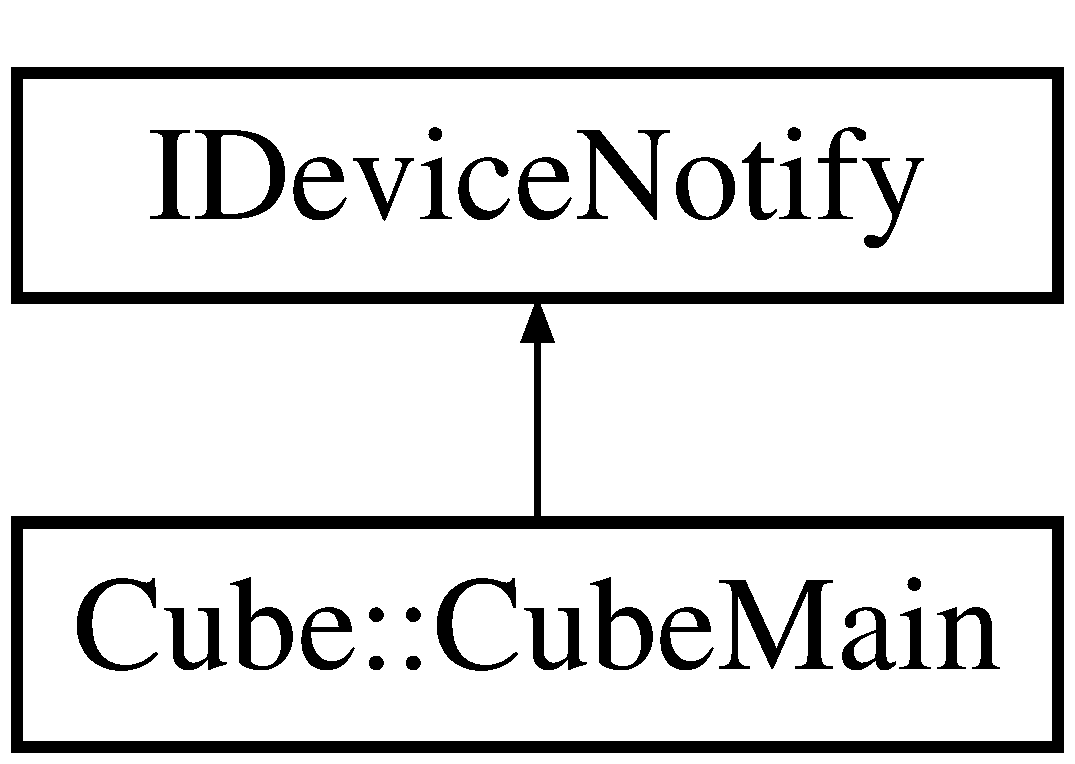
\includegraphics[height=2.000000cm]{class_cube_1_1_cube_main}
\end{center}
\end{figure}
\subsection*{Public Member Functions}
\begin{DoxyCompactItemize}
\item 
\hyperlink{class_cube_1_1_cube_main_a229d8aaeba812925915ff2c7d341ae66}{Cube\+Main} (const std\+::shared\+\_\+ptr$<$ \hyperlink{class_d_x_1_1_device_resources}{D\+X\+::\+Device\+Resources} $>$ \&device\+Resources)
\item 
\hyperlink{class_cube_1_1_cube_main_a81cc083beb265cb02e8ff2e6d7448cf0}{$\sim$\+Cube\+Main} ()
\item 
void \hyperlink{class_cube_1_1_cube_main_a584b21871de3599456d0ae51b8b1f720}{Create\+Window\+Size\+Dependent\+Resources} ()
\item 
void \hyperlink{class_cube_1_1_cube_main_a7011617c118f70dc61bfa265caf3da1a}{Update} ()
\item 
bool \hyperlink{class_cube_1_1_cube_main_a3d07f71ee05a242275b1e3f7e395d8fe}{Render} ()
\item 
virtual void \hyperlink{class_cube_1_1_cube_main_aa0d821cc48fa81986acb05bdf5d763fc}{On\+Device\+Lost} ()
\item 
virtual void \hyperlink{class_cube_1_1_cube_main_a86c314b0955424dec4cbc9734acd08ae}{On\+Device\+Restored} ()
\end{DoxyCompactItemize}


\subsection{Constructor \& Destructor Documentation}
\mbox{\Hypertarget{class_cube_1_1_cube_main_a229d8aaeba812925915ff2c7d341ae66}\label{class_cube_1_1_cube_main_a229d8aaeba812925915ff2c7d341ae66}} 
\index{Cube\+::\+Cube\+Main@{Cube\+::\+Cube\+Main}!Cube\+Main@{Cube\+Main}}
\index{Cube\+Main@{Cube\+Main}!Cube\+::\+Cube\+Main@{Cube\+::\+Cube\+Main}}
\subsubsection{\texorpdfstring{Cube\+Main()}{CubeMain()}}
{\footnotesize\ttfamily Cube\+Main\+::\+Cube\+Main (\begin{DoxyParamCaption}\item[{const std\+::shared\+\_\+ptr$<$ \hyperlink{class_d_x_1_1_device_resources}{D\+X\+::\+Device\+Resources} $>$ \&}]{device\+Resources }\end{DoxyParamCaption})}

\mbox{\Hypertarget{class_cube_1_1_cube_main_a81cc083beb265cb02e8ff2e6d7448cf0}\label{class_cube_1_1_cube_main_a81cc083beb265cb02e8ff2e6d7448cf0}} 
\index{Cube\+::\+Cube\+Main@{Cube\+::\+Cube\+Main}!````~Cube\+Main@{$\sim$\+Cube\+Main}}
\index{````~Cube\+Main@{$\sim$\+Cube\+Main}!Cube\+::\+Cube\+Main@{Cube\+::\+Cube\+Main}}
\subsubsection{\texorpdfstring{$\sim$\+Cube\+Main()}{~CubeMain()}}
{\footnotesize\ttfamily Cube\+Main\+::$\sim$\+Cube\+Main (\begin{DoxyParamCaption}{ }\end{DoxyParamCaption})}



\subsection{Member Function Documentation}
\mbox{\Hypertarget{class_cube_1_1_cube_main_a584b21871de3599456d0ae51b8b1f720}\label{class_cube_1_1_cube_main_a584b21871de3599456d0ae51b8b1f720}} 
\index{Cube\+::\+Cube\+Main@{Cube\+::\+Cube\+Main}!Create\+Window\+Size\+Dependent\+Resources@{Create\+Window\+Size\+Dependent\+Resources}}
\index{Create\+Window\+Size\+Dependent\+Resources@{Create\+Window\+Size\+Dependent\+Resources}!Cube\+::\+Cube\+Main@{Cube\+::\+Cube\+Main}}
\subsubsection{\texorpdfstring{Create\+Window\+Size\+Dependent\+Resources()}{CreateWindowSizeDependentResources()}}
{\footnotesize\ttfamily void Cube\+Main\+::\+Create\+Window\+Size\+Dependent\+Resources (\begin{DoxyParamCaption}{ }\end{DoxyParamCaption})}

\mbox{\Hypertarget{class_cube_1_1_cube_main_aa0d821cc48fa81986acb05bdf5d763fc}\label{class_cube_1_1_cube_main_aa0d821cc48fa81986acb05bdf5d763fc}} 
\index{Cube\+::\+Cube\+Main@{Cube\+::\+Cube\+Main}!On\+Device\+Lost@{On\+Device\+Lost}}
\index{On\+Device\+Lost@{On\+Device\+Lost}!Cube\+::\+Cube\+Main@{Cube\+::\+Cube\+Main}}
\subsubsection{\texorpdfstring{On\+Device\+Lost()}{OnDeviceLost()}}
{\footnotesize\ttfamily void Cube\+Main\+::\+On\+Device\+Lost (\begin{DoxyParamCaption}{ }\end{DoxyParamCaption})\hspace{0.3cm}{\ttfamily [virtual]}}

\mbox{\Hypertarget{class_cube_1_1_cube_main_a86c314b0955424dec4cbc9734acd08ae}\label{class_cube_1_1_cube_main_a86c314b0955424dec4cbc9734acd08ae}} 
\index{Cube\+::\+Cube\+Main@{Cube\+::\+Cube\+Main}!On\+Device\+Restored@{On\+Device\+Restored}}
\index{On\+Device\+Restored@{On\+Device\+Restored}!Cube\+::\+Cube\+Main@{Cube\+::\+Cube\+Main}}
\subsubsection{\texorpdfstring{On\+Device\+Restored()}{OnDeviceRestored()}}
{\footnotesize\ttfamily void Cube\+Main\+::\+On\+Device\+Restored (\begin{DoxyParamCaption}{ }\end{DoxyParamCaption})\hspace{0.3cm}{\ttfamily [virtual]}}

\mbox{\Hypertarget{class_cube_1_1_cube_main_a3d07f71ee05a242275b1e3f7e395d8fe}\label{class_cube_1_1_cube_main_a3d07f71ee05a242275b1e3f7e395d8fe}} 
\index{Cube\+::\+Cube\+Main@{Cube\+::\+Cube\+Main}!Render@{Render}}
\index{Render@{Render}!Cube\+::\+Cube\+Main@{Cube\+::\+Cube\+Main}}
\subsubsection{\texorpdfstring{Render()}{Render()}}
{\footnotesize\ttfamily bool Cube\+Main\+::\+Render (\begin{DoxyParamCaption}{ }\end{DoxyParamCaption})}

\mbox{\Hypertarget{class_cube_1_1_cube_main_a7011617c118f70dc61bfa265caf3da1a}\label{class_cube_1_1_cube_main_a7011617c118f70dc61bfa265caf3da1a}} 
\index{Cube\+::\+Cube\+Main@{Cube\+::\+Cube\+Main}!Update@{Update}}
\index{Update@{Update}!Cube\+::\+Cube\+Main@{Cube\+::\+Cube\+Main}}
\subsubsection{\texorpdfstring{Update()}{Update()}}
{\footnotesize\ttfamily void Cube\+Main\+::\+Update (\begin{DoxyParamCaption}{ }\end{DoxyParamCaption})}



The documentation for this class was generated from the following files\+:\begin{DoxyCompactItemize}
\item 
\hyperlink{_cube_main_8h}{Cube\+Main.\+h}\item 
\hyperlink{_cube_main_8cpp}{Cube\+Main.\+cpp}\end{DoxyCompactItemize}

\hypertarget{class_d_x_1_1_device_resources}{}\section{DX\+:\+:Device\+Resources Class Reference}
\label{class_d_x_1_1_device_resources}\index{D\+X\+::\+Device\+Resources@{D\+X\+::\+Device\+Resources}}


{\ttfamily \#include $<$Device\+Resources.\+h$>$}

\subsection*{Public Member Functions}
\begin{DoxyCompactItemize}
\item 
\hyperlink{class_d_x_1_1_device_resources_a7843d3aa1cd744a1502aac9124003ce5}{Device\+Resources} ()
\item 
void \hyperlink{class_d_x_1_1_device_resources_afade3e7ebc3d153276f9861fed230de9}{Set\+Window} (Windows\+::\+U\+I\+::\+Core\+::\+Core\+Window$^\wedge$ window)
\item 
void \hyperlink{class_d_x_1_1_device_resources_acc9a2f10b9169be501fad3e33e57e8da}{Set\+Logical\+Size} (Windows\+::\+Foundation\+::\+Size logical\+Size)
\item 
void \hyperlink{class_d_x_1_1_device_resources_a2359020a92c52275ec126bdf7a4ea003}{Set\+Current\+Orientation} (Windows\+::\+Graphics\+::\+Display\+::\+Display\+Orientations current\+Orientation)
\item 
void \hyperlink{class_d_x_1_1_device_resources_a82722ab9c5a11d27664e89b6a375902e}{Set\+Dpi} (float dpi)
\item 
void \hyperlink{class_d_x_1_1_device_resources_ab6976bc6f653fab6899b53a4b5308b06}{Validate\+Device} ()
\item 
void \hyperlink{class_d_x_1_1_device_resources_a31e56fca128c6e4dde8de9735dfa24c8}{Handle\+Device\+Lost} ()
\item 
void \hyperlink{class_d_x_1_1_device_resources_a89d3389fdd5d832fbf0322ad1452d08f}{Register\+Device\+Notify} (I\+Device\+Notify $\ast$device\+Notify)
\item 
void \hyperlink{class_d_x_1_1_device_resources_ac8a6eb7a3a4de63e0316382a0c3ac4a4}{Trim} ()
\item 
void \hyperlink{class_d_x_1_1_device_resources_aba74d5a48d23672e6963be1413b054d0}{Present} ()
\item 
Windows\+::\+Foundation\+::\+Size \hyperlink{class_d_x_1_1_device_resources_a098dec113d2c7614c1be33f6db3c2372}{Get\+Output\+Size} () const
\item 
Windows\+::\+Foundation\+::\+Size \hyperlink{class_d_x_1_1_device_resources_a2cf3895fe7f74f4b268d8478da492001}{Get\+Logical\+Size} () const
\item 
float \hyperlink{class_d_x_1_1_device_resources_af313814dc56d14afe8b1a02ba10d462d}{Get\+Dpi} () const
\item 
I\+D3\+D11\+Device3 $\ast$ \hyperlink{class_d_x_1_1_device_resources_aff06b3dbc3a678c38973d9b14cab98b4}{Get\+D3\+D\+Device} () const
\item 
I\+D3\+D11\+Device\+Context3 $\ast$ \hyperlink{class_d_x_1_1_device_resources_a5e9140bef766802bc08d79c1a2f422ca}{Get\+D3\+D\+Device\+Context} () const
\item 
I\+D\+X\+G\+I\+Swap\+Chain3 $\ast$ \hyperlink{class_d_x_1_1_device_resources_a5e27287ddca8d021c5ccefd46e440bea}{Get\+Swap\+Chain} () const
\item 
D3\+D\+\_\+\+F\+E\+A\+T\+U\+R\+E\+\_\+\+L\+E\+V\+EL \hyperlink{class_d_x_1_1_device_resources_a2fcb785972e693d3d8cb711a09cb9f1e}{Get\+Device\+Feature\+Level} () const
\item 
I\+D3\+D11\+Render\+Target\+View1 $\ast$ \hyperlink{class_d_x_1_1_device_resources_ac76b0cfbc12336b39122878c0b875af7}{Get\+Back\+Buffer\+Render\+Target\+View} () const
\item 
I\+D3\+D11\+Depth\+Stencil\+View $\ast$ \hyperlink{class_d_x_1_1_device_resources_a1d9c271bdc8163ee77a175e305fbfb88}{Get\+Depth\+Stencil\+View} () const
\item 
D3\+D11\+\_\+\+V\+I\+E\+W\+P\+O\+RT \hyperlink{class_d_x_1_1_device_resources_aaaadbe1b6ab02879f493914d4440c0c6}{Get\+Screen\+Viewport} () const
\item 
Direct\+X\+::\+X\+M\+F\+L\+O\+A\+T4\+X4 \hyperlink{class_d_x_1_1_device_resources_aaedd593f914988c1aee0712ada59032b}{Get\+Orientation\+Transform3D} () const
\item 
I\+D2\+D1\+Factory3 $\ast$ \hyperlink{class_d_x_1_1_device_resources_a5ccb7b47646cb49a58051ef6b0b90614}{Get\+D2\+D\+Factory} () const
\item 
I\+D2\+D1\+Device2 $\ast$ \hyperlink{class_d_x_1_1_device_resources_a95a773d012e00d4fc6c62ee8b09324a9}{Get\+D2\+D\+Device} () const
\item 
I\+D2\+D1\+Device\+Context2 $\ast$ \hyperlink{class_d_x_1_1_device_resources_a214cafc8d9a6b7bad7394c2a2270aff6}{Get\+D2\+D\+Device\+Context} () const
\item 
I\+D2\+D1\+Bitmap1 $\ast$ \hyperlink{class_d_x_1_1_device_resources_a249227733502bf12f78c2e43875583ee}{Get\+D2\+D\+Target\+Bitmap} () const
\item 
I\+D\+Write\+Factory3 $\ast$ \hyperlink{class_d_x_1_1_device_resources_a12dd3a477131220352b1ade8808d5704}{Get\+D\+Write\+Factory} () const
\item 
I\+W\+I\+C\+Imaging\+Factory2 $\ast$ \hyperlink{class_d_x_1_1_device_resources_a1f299821812c1943c0230903e0500e39}{Get\+Wic\+Imaging\+Factory} () const
\item 
D2\+D1\+::\+Matrix3x2F \hyperlink{class_d_x_1_1_device_resources_a428f59800d7616836359026496d901f9}{Get\+Orientation\+Transform2D} () const
\end{DoxyCompactItemize}


\subsection{Constructor \& Destructor Documentation}
\mbox{\Hypertarget{class_d_x_1_1_device_resources_a7843d3aa1cd744a1502aac9124003ce5}\label{class_d_x_1_1_device_resources_a7843d3aa1cd744a1502aac9124003ce5}} 
\index{D\+X\+::\+Device\+Resources@{D\+X\+::\+Device\+Resources}!Device\+Resources@{Device\+Resources}}
\index{Device\+Resources@{Device\+Resources}!D\+X\+::\+Device\+Resources@{D\+X\+::\+Device\+Resources}}
\subsubsection{\texorpdfstring{Device\+Resources()}{DeviceResources()}}
{\footnotesize\ttfamily D\+X\+::\+Device\+Resources\+::\+Device\+Resources (\begin{DoxyParamCaption}{ }\end{DoxyParamCaption})}



\subsection{Member Function Documentation}
\mbox{\Hypertarget{class_d_x_1_1_device_resources_ac76b0cfbc12336b39122878c0b875af7}\label{class_d_x_1_1_device_resources_ac76b0cfbc12336b39122878c0b875af7}} 
\index{D\+X\+::\+Device\+Resources@{D\+X\+::\+Device\+Resources}!Get\+Back\+Buffer\+Render\+Target\+View@{Get\+Back\+Buffer\+Render\+Target\+View}}
\index{Get\+Back\+Buffer\+Render\+Target\+View@{Get\+Back\+Buffer\+Render\+Target\+View}!D\+X\+::\+Device\+Resources@{D\+X\+::\+Device\+Resources}}
\subsubsection{\texorpdfstring{Get\+Back\+Buffer\+Render\+Target\+View()}{GetBackBufferRenderTargetView()}}
{\footnotesize\ttfamily I\+D3\+D11\+Render\+Target\+View1$\ast$ D\+X\+::\+Device\+Resources\+::\+Get\+Back\+Buffer\+Render\+Target\+View (\begin{DoxyParamCaption}{ }\end{DoxyParamCaption}) const\hspace{0.3cm}{\ttfamily [inline]}}

\mbox{\Hypertarget{class_d_x_1_1_device_resources_a95a773d012e00d4fc6c62ee8b09324a9}\label{class_d_x_1_1_device_resources_a95a773d012e00d4fc6c62ee8b09324a9}} 
\index{D\+X\+::\+Device\+Resources@{D\+X\+::\+Device\+Resources}!Get\+D2\+D\+Device@{Get\+D2\+D\+Device}}
\index{Get\+D2\+D\+Device@{Get\+D2\+D\+Device}!D\+X\+::\+Device\+Resources@{D\+X\+::\+Device\+Resources}}
\subsubsection{\texorpdfstring{Get\+D2\+D\+Device()}{GetD2DDevice()}}
{\footnotesize\ttfamily I\+D2\+D1\+Device2$\ast$ D\+X\+::\+Device\+Resources\+::\+Get\+D2\+D\+Device (\begin{DoxyParamCaption}{ }\end{DoxyParamCaption}) const\hspace{0.3cm}{\ttfamily [inline]}}

\mbox{\Hypertarget{class_d_x_1_1_device_resources_a214cafc8d9a6b7bad7394c2a2270aff6}\label{class_d_x_1_1_device_resources_a214cafc8d9a6b7bad7394c2a2270aff6}} 
\index{D\+X\+::\+Device\+Resources@{D\+X\+::\+Device\+Resources}!Get\+D2\+D\+Device\+Context@{Get\+D2\+D\+Device\+Context}}
\index{Get\+D2\+D\+Device\+Context@{Get\+D2\+D\+Device\+Context}!D\+X\+::\+Device\+Resources@{D\+X\+::\+Device\+Resources}}
\subsubsection{\texorpdfstring{Get\+D2\+D\+Device\+Context()}{GetD2DDeviceContext()}}
{\footnotesize\ttfamily I\+D2\+D1\+Device\+Context2$\ast$ D\+X\+::\+Device\+Resources\+::\+Get\+D2\+D\+Device\+Context (\begin{DoxyParamCaption}{ }\end{DoxyParamCaption}) const\hspace{0.3cm}{\ttfamily [inline]}}

\mbox{\Hypertarget{class_d_x_1_1_device_resources_a5ccb7b47646cb49a58051ef6b0b90614}\label{class_d_x_1_1_device_resources_a5ccb7b47646cb49a58051ef6b0b90614}} 
\index{D\+X\+::\+Device\+Resources@{D\+X\+::\+Device\+Resources}!Get\+D2\+D\+Factory@{Get\+D2\+D\+Factory}}
\index{Get\+D2\+D\+Factory@{Get\+D2\+D\+Factory}!D\+X\+::\+Device\+Resources@{D\+X\+::\+Device\+Resources}}
\subsubsection{\texorpdfstring{Get\+D2\+D\+Factory()}{GetD2DFactory()}}
{\footnotesize\ttfamily I\+D2\+D1\+Factory3$\ast$ D\+X\+::\+Device\+Resources\+::\+Get\+D2\+D\+Factory (\begin{DoxyParamCaption}{ }\end{DoxyParamCaption}) const\hspace{0.3cm}{\ttfamily [inline]}}

\mbox{\Hypertarget{class_d_x_1_1_device_resources_a249227733502bf12f78c2e43875583ee}\label{class_d_x_1_1_device_resources_a249227733502bf12f78c2e43875583ee}} 
\index{D\+X\+::\+Device\+Resources@{D\+X\+::\+Device\+Resources}!Get\+D2\+D\+Target\+Bitmap@{Get\+D2\+D\+Target\+Bitmap}}
\index{Get\+D2\+D\+Target\+Bitmap@{Get\+D2\+D\+Target\+Bitmap}!D\+X\+::\+Device\+Resources@{D\+X\+::\+Device\+Resources}}
\subsubsection{\texorpdfstring{Get\+D2\+D\+Target\+Bitmap()}{GetD2DTargetBitmap()}}
{\footnotesize\ttfamily I\+D2\+D1\+Bitmap1$\ast$ D\+X\+::\+Device\+Resources\+::\+Get\+D2\+D\+Target\+Bitmap (\begin{DoxyParamCaption}{ }\end{DoxyParamCaption}) const\hspace{0.3cm}{\ttfamily [inline]}}

\mbox{\Hypertarget{class_d_x_1_1_device_resources_aff06b3dbc3a678c38973d9b14cab98b4}\label{class_d_x_1_1_device_resources_aff06b3dbc3a678c38973d9b14cab98b4}} 
\index{D\+X\+::\+Device\+Resources@{D\+X\+::\+Device\+Resources}!Get\+D3\+D\+Device@{Get\+D3\+D\+Device}}
\index{Get\+D3\+D\+Device@{Get\+D3\+D\+Device}!D\+X\+::\+Device\+Resources@{D\+X\+::\+Device\+Resources}}
\subsubsection{\texorpdfstring{Get\+D3\+D\+Device()}{GetD3DDevice()}}
{\footnotesize\ttfamily I\+D3\+D11\+Device3$\ast$ D\+X\+::\+Device\+Resources\+::\+Get\+D3\+D\+Device (\begin{DoxyParamCaption}{ }\end{DoxyParamCaption}) const\hspace{0.3cm}{\ttfamily [inline]}}

\mbox{\Hypertarget{class_d_x_1_1_device_resources_a5e9140bef766802bc08d79c1a2f422ca}\label{class_d_x_1_1_device_resources_a5e9140bef766802bc08d79c1a2f422ca}} 
\index{D\+X\+::\+Device\+Resources@{D\+X\+::\+Device\+Resources}!Get\+D3\+D\+Device\+Context@{Get\+D3\+D\+Device\+Context}}
\index{Get\+D3\+D\+Device\+Context@{Get\+D3\+D\+Device\+Context}!D\+X\+::\+Device\+Resources@{D\+X\+::\+Device\+Resources}}
\subsubsection{\texorpdfstring{Get\+D3\+D\+Device\+Context()}{GetD3DDeviceContext()}}
{\footnotesize\ttfamily I\+D3\+D11\+Device\+Context3$\ast$ D\+X\+::\+Device\+Resources\+::\+Get\+D3\+D\+Device\+Context (\begin{DoxyParamCaption}{ }\end{DoxyParamCaption}) const\hspace{0.3cm}{\ttfamily [inline]}}

\mbox{\Hypertarget{class_d_x_1_1_device_resources_a1d9c271bdc8163ee77a175e305fbfb88}\label{class_d_x_1_1_device_resources_a1d9c271bdc8163ee77a175e305fbfb88}} 
\index{D\+X\+::\+Device\+Resources@{D\+X\+::\+Device\+Resources}!Get\+Depth\+Stencil\+View@{Get\+Depth\+Stencil\+View}}
\index{Get\+Depth\+Stencil\+View@{Get\+Depth\+Stencil\+View}!D\+X\+::\+Device\+Resources@{D\+X\+::\+Device\+Resources}}
\subsubsection{\texorpdfstring{Get\+Depth\+Stencil\+View()}{GetDepthStencilView()}}
{\footnotesize\ttfamily I\+D3\+D11\+Depth\+Stencil\+View$\ast$ D\+X\+::\+Device\+Resources\+::\+Get\+Depth\+Stencil\+View (\begin{DoxyParamCaption}{ }\end{DoxyParamCaption}) const\hspace{0.3cm}{\ttfamily [inline]}}

\mbox{\Hypertarget{class_d_x_1_1_device_resources_a2fcb785972e693d3d8cb711a09cb9f1e}\label{class_d_x_1_1_device_resources_a2fcb785972e693d3d8cb711a09cb9f1e}} 
\index{D\+X\+::\+Device\+Resources@{D\+X\+::\+Device\+Resources}!Get\+Device\+Feature\+Level@{Get\+Device\+Feature\+Level}}
\index{Get\+Device\+Feature\+Level@{Get\+Device\+Feature\+Level}!D\+X\+::\+Device\+Resources@{D\+X\+::\+Device\+Resources}}
\subsubsection{\texorpdfstring{Get\+Device\+Feature\+Level()}{GetDeviceFeatureLevel()}}
{\footnotesize\ttfamily D3\+D\+\_\+\+F\+E\+A\+T\+U\+R\+E\+\_\+\+L\+E\+V\+EL D\+X\+::\+Device\+Resources\+::\+Get\+Device\+Feature\+Level (\begin{DoxyParamCaption}{ }\end{DoxyParamCaption}) const\hspace{0.3cm}{\ttfamily [inline]}}

\mbox{\Hypertarget{class_d_x_1_1_device_resources_af313814dc56d14afe8b1a02ba10d462d}\label{class_d_x_1_1_device_resources_af313814dc56d14afe8b1a02ba10d462d}} 
\index{D\+X\+::\+Device\+Resources@{D\+X\+::\+Device\+Resources}!Get\+Dpi@{Get\+Dpi}}
\index{Get\+Dpi@{Get\+Dpi}!D\+X\+::\+Device\+Resources@{D\+X\+::\+Device\+Resources}}
\subsubsection{\texorpdfstring{Get\+Dpi()}{GetDpi()}}
{\footnotesize\ttfamily float D\+X\+::\+Device\+Resources\+::\+Get\+Dpi (\begin{DoxyParamCaption}{ }\end{DoxyParamCaption}) const\hspace{0.3cm}{\ttfamily [inline]}}

\mbox{\Hypertarget{class_d_x_1_1_device_resources_a12dd3a477131220352b1ade8808d5704}\label{class_d_x_1_1_device_resources_a12dd3a477131220352b1ade8808d5704}} 
\index{D\+X\+::\+Device\+Resources@{D\+X\+::\+Device\+Resources}!Get\+D\+Write\+Factory@{Get\+D\+Write\+Factory}}
\index{Get\+D\+Write\+Factory@{Get\+D\+Write\+Factory}!D\+X\+::\+Device\+Resources@{D\+X\+::\+Device\+Resources}}
\subsubsection{\texorpdfstring{Get\+D\+Write\+Factory()}{GetDWriteFactory()}}
{\footnotesize\ttfamily I\+D\+Write\+Factory3$\ast$ D\+X\+::\+Device\+Resources\+::\+Get\+D\+Write\+Factory (\begin{DoxyParamCaption}{ }\end{DoxyParamCaption}) const\hspace{0.3cm}{\ttfamily [inline]}}

\mbox{\Hypertarget{class_d_x_1_1_device_resources_a2cf3895fe7f74f4b268d8478da492001}\label{class_d_x_1_1_device_resources_a2cf3895fe7f74f4b268d8478da492001}} 
\index{D\+X\+::\+Device\+Resources@{D\+X\+::\+Device\+Resources}!Get\+Logical\+Size@{Get\+Logical\+Size}}
\index{Get\+Logical\+Size@{Get\+Logical\+Size}!D\+X\+::\+Device\+Resources@{D\+X\+::\+Device\+Resources}}
\subsubsection{\texorpdfstring{Get\+Logical\+Size()}{GetLogicalSize()}}
{\footnotesize\ttfamily Windows\+::\+Foundation\+::\+Size D\+X\+::\+Device\+Resources\+::\+Get\+Logical\+Size (\begin{DoxyParamCaption}{ }\end{DoxyParamCaption}) const\hspace{0.3cm}{\ttfamily [inline]}}

\mbox{\Hypertarget{class_d_x_1_1_device_resources_a428f59800d7616836359026496d901f9}\label{class_d_x_1_1_device_resources_a428f59800d7616836359026496d901f9}} 
\index{D\+X\+::\+Device\+Resources@{D\+X\+::\+Device\+Resources}!Get\+Orientation\+Transform2D@{Get\+Orientation\+Transform2D}}
\index{Get\+Orientation\+Transform2D@{Get\+Orientation\+Transform2D}!D\+X\+::\+Device\+Resources@{D\+X\+::\+Device\+Resources}}
\subsubsection{\texorpdfstring{Get\+Orientation\+Transform2\+D()}{GetOrientationTransform2D()}}
{\footnotesize\ttfamily D2\+D1\+::\+Matrix3x2F D\+X\+::\+Device\+Resources\+::\+Get\+Orientation\+Transform2D (\begin{DoxyParamCaption}{ }\end{DoxyParamCaption}) const\hspace{0.3cm}{\ttfamily [inline]}}

\mbox{\Hypertarget{class_d_x_1_1_device_resources_aaedd593f914988c1aee0712ada59032b}\label{class_d_x_1_1_device_resources_aaedd593f914988c1aee0712ada59032b}} 
\index{D\+X\+::\+Device\+Resources@{D\+X\+::\+Device\+Resources}!Get\+Orientation\+Transform3D@{Get\+Orientation\+Transform3D}}
\index{Get\+Orientation\+Transform3D@{Get\+Orientation\+Transform3D}!D\+X\+::\+Device\+Resources@{D\+X\+::\+Device\+Resources}}
\subsubsection{\texorpdfstring{Get\+Orientation\+Transform3\+D()}{GetOrientationTransform3D()}}
{\footnotesize\ttfamily Direct\+X\+::\+X\+M\+F\+L\+O\+A\+T4\+X4 D\+X\+::\+Device\+Resources\+::\+Get\+Orientation\+Transform3D (\begin{DoxyParamCaption}{ }\end{DoxyParamCaption}) const\hspace{0.3cm}{\ttfamily [inline]}}

\mbox{\Hypertarget{class_d_x_1_1_device_resources_a098dec113d2c7614c1be33f6db3c2372}\label{class_d_x_1_1_device_resources_a098dec113d2c7614c1be33f6db3c2372}} 
\index{D\+X\+::\+Device\+Resources@{D\+X\+::\+Device\+Resources}!Get\+Output\+Size@{Get\+Output\+Size}}
\index{Get\+Output\+Size@{Get\+Output\+Size}!D\+X\+::\+Device\+Resources@{D\+X\+::\+Device\+Resources}}
\subsubsection{\texorpdfstring{Get\+Output\+Size()}{GetOutputSize()}}
{\footnotesize\ttfamily Windows\+::\+Foundation\+::\+Size D\+X\+::\+Device\+Resources\+::\+Get\+Output\+Size (\begin{DoxyParamCaption}{ }\end{DoxyParamCaption}) const\hspace{0.3cm}{\ttfamily [inline]}}

\mbox{\Hypertarget{class_d_x_1_1_device_resources_aaaadbe1b6ab02879f493914d4440c0c6}\label{class_d_x_1_1_device_resources_aaaadbe1b6ab02879f493914d4440c0c6}} 
\index{D\+X\+::\+Device\+Resources@{D\+X\+::\+Device\+Resources}!Get\+Screen\+Viewport@{Get\+Screen\+Viewport}}
\index{Get\+Screen\+Viewport@{Get\+Screen\+Viewport}!D\+X\+::\+Device\+Resources@{D\+X\+::\+Device\+Resources}}
\subsubsection{\texorpdfstring{Get\+Screen\+Viewport()}{GetScreenViewport()}}
{\footnotesize\ttfamily D3\+D11\+\_\+\+V\+I\+E\+W\+P\+O\+RT D\+X\+::\+Device\+Resources\+::\+Get\+Screen\+Viewport (\begin{DoxyParamCaption}{ }\end{DoxyParamCaption}) const\hspace{0.3cm}{\ttfamily [inline]}}

\mbox{\Hypertarget{class_d_x_1_1_device_resources_a5e27287ddca8d021c5ccefd46e440bea}\label{class_d_x_1_1_device_resources_a5e27287ddca8d021c5ccefd46e440bea}} 
\index{D\+X\+::\+Device\+Resources@{D\+X\+::\+Device\+Resources}!Get\+Swap\+Chain@{Get\+Swap\+Chain}}
\index{Get\+Swap\+Chain@{Get\+Swap\+Chain}!D\+X\+::\+Device\+Resources@{D\+X\+::\+Device\+Resources}}
\subsubsection{\texorpdfstring{Get\+Swap\+Chain()}{GetSwapChain()}}
{\footnotesize\ttfamily I\+D\+X\+G\+I\+Swap\+Chain3$\ast$ D\+X\+::\+Device\+Resources\+::\+Get\+Swap\+Chain (\begin{DoxyParamCaption}{ }\end{DoxyParamCaption}) const\hspace{0.3cm}{\ttfamily [inline]}}

\mbox{\Hypertarget{class_d_x_1_1_device_resources_a1f299821812c1943c0230903e0500e39}\label{class_d_x_1_1_device_resources_a1f299821812c1943c0230903e0500e39}} 
\index{D\+X\+::\+Device\+Resources@{D\+X\+::\+Device\+Resources}!Get\+Wic\+Imaging\+Factory@{Get\+Wic\+Imaging\+Factory}}
\index{Get\+Wic\+Imaging\+Factory@{Get\+Wic\+Imaging\+Factory}!D\+X\+::\+Device\+Resources@{D\+X\+::\+Device\+Resources}}
\subsubsection{\texorpdfstring{Get\+Wic\+Imaging\+Factory()}{GetWicImagingFactory()}}
{\footnotesize\ttfamily I\+W\+I\+C\+Imaging\+Factory2$\ast$ D\+X\+::\+Device\+Resources\+::\+Get\+Wic\+Imaging\+Factory (\begin{DoxyParamCaption}{ }\end{DoxyParamCaption}) const\hspace{0.3cm}{\ttfamily [inline]}}

\mbox{\Hypertarget{class_d_x_1_1_device_resources_a31e56fca128c6e4dde8de9735dfa24c8}\label{class_d_x_1_1_device_resources_a31e56fca128c6e4dde8de9735dfa24c8}} 
\index{D\+X\+::\+Device\+Resources@{D\+X\+::\+Device\+Resources}!Handle\+Device\+Lost@{Handle\+Device\+Lost}}
\index{Handle\+Device\+Lost@{Handle\+Device\+Lost}!D\+X\+::\+Device\+Resources@{D\+X\+::\+Device\+Resources}}
\subsubsection{\texorpdfstring{Handle\+Device\+Lost()}{HandleDeviceLost()}}
{\footnotesize\ttfamily void D\+X\+::\+Device\+Resources\+::\+Handle\+Device\+Lost (\begin{DoxyParamCaption}{ }\end{DoxyParamCaption})}

\mbox{\Hypertarget{class_d_x_1_1_device_resources_aba74d5a48d23672e6963be1413b054d0}\label{class_d_x_1_1_device_resources_aba74d5a48d23672e6963be1413b054d0}} 
\index{D\+X\+::\+Device\+Resources@{D\+X\+::\+Device\+Resources}!Present@{Present}}
\index{Present@{Present}!D\+X\+::\+Device\+Resources@{D\+X\+::\+Device\+Resources}}
\subsubsection{\texorpdfstring{Present()}{Present()}}
{\footnotesize\ttfamily void D\+X\+::\+Device\+Resources\+::\+Present (\begin{DoxyParamCaption}{ }\end{DoxyParamCaption})}

\mbox{\Hypertarget{class_d_x_1_1_device_resources_a89d3389fdd5d832fbf0322ad1452d08f}\label{class_d_x_1_1_device_resources_a89d3389fdd5d832fbf0322ad1452d08f}} 
\index{D\+X\+::\+Device\+Resources@{D\+X\+::\+Device\+Resources}!Register\+Device\+Notify@{Register\+Device\+Notify}}
\index{Register\+Device\+Notify@{Register\+Device\+Notify}!D\+X\+::\+Device\+Resources@{D\+X\+::\+Device\+Resources}}
\subsubsection{\texorpdfstring{Register\+Device\+Notify()}{RegisterDeviceNotify()}}
{\footnotesize\ttfamily void D\+X\+::\+Device\+Resources\+::\+Register\+Device\+Notify (\begin{DoxyParamCaption}\item[{D\+X\+::\+I\+Device\+Notify $\ast$}]{device\+Notify }\end{DoxyParamCaption})}

\mbox{\Hypertarget{class_d_x_1_1_device_resources_a2359020a92c52275ec126bdf7a4ea003}\label{class_d_x_1_1_device_resources_a2359020a92c52275ec126bdf7a4ea003}} 
\index{D\+X\+::\+Device\+Resources@{D\+X\+::\+Device\+Resources}!Set\+Current\+Orientation@{Set\+Current\+Orientation}}
\index{Set\+Current\+Orientation@{Set\+Current\+Orientation}!D\+X\+::\+Device\+Resources@{D\+X\+::\+Device\+Resources}}
\subsubsection{\texorpdfstring{Set\+Current\+Orientation()}{SetCurrentOrientation()}}
{\footnotesize\ttfamily void D\+X\+::\+Device\+Resources\+::\+Set\+Current\+Orientation (\begin{DoxyParamCaption}\item[{Windows\+::\+Graphics\+::\+Display\+::\+Display\+Orientations}]{current\+Orientation }\end{DoxyParamCaption})}

\mbox{\Hypertarget{class_d_x_1_1_device_resources_a82722ab9c5a11d27664e89b6a375902e}\label{class_d_x_1_1_device_resources_a82722ab9c5a11d27664e89b6a375902e}} 
\index{D\+X\+::\+Device\+Resources@{D\+X\+::\+Device\+Resources}!Set\+Dpi@{Set\+Dpi}}
\index{Set\+Dpi@{Set\+Dpi}!D\+X\+::\+Device\+Resources@{D\+X\+::\+Device\+Resources}}
\subsubsection{\texorpdfstring{Set\+Dpi()}{SetDpi()}}
{\footnotesize\ttfamily void D\+X\+::\+Device\+Resources\+::\+Set\+Dpi (\begin{DoxyParamCaption}\item[{float}]{dpi }\end{DoxyParamCaption})}

\mbox{\Hypertarget{class_d_x_1_1_device_resources_acc9a2f10b9169be501fad3e33e57e8da}\label{class_d_x_1_1_device_resources_acc9a2f10b9169be501fad3e33e57e8da}} 
\index{D\+X\+::\+Device\+Resources@{D\+X\+::\+Device\+Resources}!Set\+Logical\+Size@{Set\+Logical\+Size}}
\index{Set\+Logical\+Size@{Set\+Logical\+Size}!D\+X\+::\+Device\+Resources@{D\+X\+::\+Device\+Resources}}
\subsubsection{\texorpdfstring{Set\+Logical\+Size()}{SetLogicalSize()}}
{\footnotesize\ttfamily void D\+X\+::\+Device\+Resources\+::\+Set\+Logical\+Size (\begin{DoxyParamCaption}\item[{Windows\+::\+Foundation\+::\+Size}]{logical\+Size }\end{DoxyParamCaption})}

\mbox{\Hypertarget{class_d_x_1_1_device_resources_afade3e7ebc3d153276f9861fed230de9}\label{class_d_x_1_1_device_resources_afade3e7ebc3d153276f9861fed230de9}} 
\index{D\+X\+::\+Device\+Resources@{D\+X\+::\+Device\+Resources}!Set\+Window@{Set\+Window}}
\index{Set\+Window@{Set\+Window}!D\+X\+::\+Device\+Resources@{D\+X\+::\+Device\+Resources}}
\subsubsection{\texorpdfstring{Set\+Window()}{SetWindow()}}
{\footnotesize\ttfamily void D\+X\+::\+Device\+Resources\+::\+Set\+Window (\begin{DoxyParamCaption}\item[{Windows\+::\+U\+I\+::\+Core\+::\+Core\+Window$^\wedge$}]{window }\end{DoxyParamCaption})}

\mbox{\Hypertarget{class_d_x_1_1_device_resources_ac8a6eb7a3a4de63e0316382a0c3ac4a4}\label{class_d_x_1_1_device_resources_ac8a6eb7a3a4de63e0316382a0c3ac4a4}} 
\index{D\+X\+::\+Device\+Resources@{D\+X\+::\+Device\+Resources}!Trim@{Trim}}
\index{Trim@{Trim}!D\+X\+::\+Device\+Resources@{D\+X\+::\+Device\+Resources}}
\subsubsection{\texorpdfstring{Trim()}{Trim()}}
{\footnotesize\ttfamily void D\+X\+::\+Device\+Resources\+::\+Trim (\begin{DoxyParamCaption}{ }\end{DoxyParamCaption})}

\mbox{\Hypertarget{class_d_x_1_1_device_resources_ab6976bc6f653fab6899b53a4b5308b06}\label{class_d_x_1_1_device_resources_ab6976bc6f653fab6899b53a4b5308b06}} 
\index{D\+X\+::\+Device\+Resources@{D\+X\+::\+Device\+Resources}!Validate\+Device@{Validate\+Device}}
\index{Validate\+Device@{Validate\+Device}!D\+X\+::\+Device\+Resources@{D\+X\+::\+Device\+Resources}}
\subsubsection{\texorpdfstring{Validate\+Device()}{ValidateDevice()}}
{\footnotesize\ttfamily void D\+X\+::\+Device\+Resources\+::\+Validate\+Device (\begin{DoxyParamCaption}{ }\end{DoxyParamCaption})}



The documentation for this class was generated from the following files\+:\begin{DoxyCompactItemize}
\item 
Common/\hyperlink{_device_resources_8h}{Device\+Resources.\+h}\item 
Common/\hyperlink{_device_resources_8cpp}{Device\+Resources.\+cpp}\end{DoxyCompactItemize}

\hypertarget{struct_cube_1_1_model_view_projection_constant_buffer}{}\section{Cube\+:\+:Model\+View\+Projection\+Constant\+Buffer Struct Reference}
\label{struct_cube_1_1_model_view_projection_constant_buffer}\index{Cube\+::\+Model\+View\+Projection\+Constant\+Buffer@{Cube\+::\+Model\+View\+Projection\+Constant\+Buffer}}


{\ttfamily \#include $<$Shader\+Structures.\+h$>$}

\subsection*{Public Attributes}
\begin{DoxyCompactItemize}
\item 
Direct\+X\+::\+X\+M\+F\+L\+O\+A\+T4\+X4 \hyperlink{struct_cube_1_1_model_view_projection_constant_buffer_a1a7ffc14e72945bd0ece96ef5954d9a5}{model}
\item 
Direct\+X\+::\+X\+M\+F\+L\+O\+A\+T4\+X4 \hyperlink{struct_cube_1_1_model_view_projection_constant_buffer_a43f3448b822ee84ab49e40cbf74cd3e1}{view}
\item 
Direct\+X\+::\+X\+M\+F\+L\+O\+A\+T4\+X4 \hyperlink{struct_cube_1_1_model_view_projection_constant_buffer_a81ad61fe5f418f01da4fd9667975a6e4}{projection}
\item 
Direct\+X\+::\+X\+M\+F\+L\+O\+A\+T4 \hyperlink{struct_cube_1_1_model_view_projection_constant_buffer_ac6b5249e850b2f3deef3d8fc20614e85}{vec\+\_\+light}
\item 
Direct\+X\+::\+X\+M\+F\+L\+O\+A\+T4 \hyperlink{struct_cube_1_1_model_view_projection_constant_buffer_ab67504141f43910f88d78ebebf0f30a0}{view\+Pos}
\end{DoxyCompactItemize}


\subsection{Member Data Documentation}
\mbox{\Hypertarget{struct_cube_1_1_model_view_projection_constant_buffer_a1a7ffc14e72945bd0ece96ef5954d9a5}\label{struct_cube_1_1_model_view_projection_constant_buffer_a1a7ffc14e72945bd0ece96ef5954d9a5}} 
\index{Cube\+::\+Model\+View\+Projection\+Constant\+Buffer@{Cube\+::\+Model\+View\+Projection\+Constant\+Buffer}!model@{model}}
\index{model@{model}!Cube\+::\+Model\+View\+Projection\+Constant\+Buffer@{Cube\+::\+Model\+View\+Projection\+Constant\+Buffer}}
\subsubsection{\texorpdfstring{model}{model}}
{\footnotesize\ttfamily Direct\+X\+::\+X\+M\+F\+L\+O\+A\+T4\+X4 Cube\+::\+Model\+View\+Projection\+Constant\+Buffer\+::model}

\mbox{\Hypertarget{struct_cube_1_1_model_view_projection_constant_buffer_a81ad61fe5f418f01da4fd9667975a6e4}\label{struct_cube_1_1_model_view_projection_constant_buffer_a81ad61fe5f418f01da4fd9667975a6e4}} 
\index{Cube\+::\+Model\+View\+Projection\+Constant\+Buffer@{Cube\+::\+Model\+View\+Projection\+Constant\+Buffer}!projection@{projection}}
\index{projection@{projection}!Cube\+::\+Model\+View\+Projection\+Constant\+Buffer@{Cube\+::\+Model\+View\+Projection\+Constant\+Buffer}}
\subsubsection{\texorpdfstring{projection}{projection}}
{\footnotesize\ttfamily Direct\+X\+::\+X\+M\+F\+L\+O\+A\+T4\+X4 Cube\+::\+Model\+View\+Projection\+Constant\+Buffer\+::projection}

\mbox{\Hypertarget{struct_cube_1_1_model_view_projection_constant_buffer_ac6b5249e850b2f3deef3d8fc20614e85}\label{struct_cube_1_1_model_view_projection_constant_buffer_ac6b5249e850b2f3deef3d8fc20614e85}} 
\index{Cube\+::\+Model\+View\+Projection\+Constant\+Buffer@{Cube\+::\+Model\+View\+Projection\+Constant\+Buffer}!vec\+\_\+light@{vec\+\_\+light}}
\index{vec\+\_\+light@{vec\+\_\+light}!Cube\+::\+Model\+View\+Projection\+Constant\+Buffer@{Cube\+::\+Model\+View\+Projection\+Constant\+Buffer}}
\subsubsection{\texorpdfstring{vec\+\_\+light}{vec\_light}}
{\footnotesize\ttfamily Direct\+X\+::\+X\+M\+F\+L\+O\+A\+T4 Cube\+::\+Model\+View\+Projection\+Constant\+Buffer\+::vec\+\_\+light}

\mbox{\Hypertarget{struct_cube_1_1_model_view_projection_constant_buffer_a43f3448b822ee84ab49e40cbf74cd3e1}\label{struct_cube_1_1_model_view_projection_constant_buffer_a43f3448b822ee84ab49e40cbf74cd3e1}} 
\index{Cube\+::\+Model\+View\+Projection\+Constant\+Buffer@{Cube\+::\+Model\+View\+Projection\+Constant\+Buffer}!view@{view}}
\index{view@{view}!Cube\+::\+Model\+View\+Projection\+Constant\+Buffer@{Cube\+::\+Model\+View\+Projection\+Constant\+Buffer}}
\subsubsection{\texorpdfstring{view}{view}}
{\footnotesize\ttfamily Direct\+X\+::\+X\+M\+F\+L\+O\+A\+T4\+X4 Cube\+::\+Model\+View\+Projection\+Constant\+Buffer\+::view}

\mbox{\Hypertarget{struct_cube_1_1_model_view_projection_constant_buffer_ab67504141f43910f88d78ebebf0f30a0}\label{struct_cube_1_1_model_view_projection_constant_buffer_ab67504141f43910f88d78ebebf0f30a0}} 
\index{Cube\+::\+Model\+View\+Projection\+Constant\+Buffer@{Cube\+::\+Model\+View\+Projection\+Constant\+Buffer}!view\+Pos@{view\+Pos}}
\index{view\+Pos@{view\+Pos}!Cube\+::\+Model\+View\+Projection\+Constant\+Buffer@{Cube\+::\+Model\+View\+Projection\+Constant\+Buffer}}
\subsubsection{\texorpdfstring{view\+Pos}{viewPos}}
{\footnotesize\ttfamily Direct\+X\+::\+X\+M\+F\+L\+O\+A\+T4 Cube\+::\+Model\+View\+Projection\+Constant\+Buffer\+::view\+Pos}



The documentation for this struct was generated from the following file\+:\begin{DoxyCompactItemize}
\item 
Content/\hyperlink{_shader_structures_8h}{Shader\+Structures.\+h}\end{DoxyCompactItemize}

\hypertarget{class_cube_1_1_sample3_d_scene_renderer}{}\section{Cube\+:\+:Sample3\+D\+Scene\+Renderer Class Reference}
\label{class_cube_1_1_sample3_d_scene_renderer}\index{Cube\+::\+Sample3\+D\+Scene\+Renderer@{Cube\+::\+Sample3\+D\+Scene\+Renderer}}


{\ttfamily \#include $<$Sample3\+D\+Scene\+Renderer.\+h$>$}

\subsection*{Public Member Functions}
\begin{DoxyCompactItemize}
\item 
\hyperlink{class_cube_1_1_sample3_d_scene_renderer_a7909da3aa7c4ba6361661f2ece368a2d}{Sample3\+D\+Scene\+Renderer} (const std\+::shared\+\_\+ptr$<$ \hyperlink{class_d_x_1_1_device_resources}{D\+X\+::\+Device\+Resources} $>$ \&device\+Resources)
\item 
void \hyperlink{class_cube_1_1_sample3_d_scene_renderer_ac5c1b9d012427c30e3effcf67ff8f25e}{Create\+Device\+Dependent\+Resources} ()
\item 
void \hyperlink{class_cube_1_1_sample3_d_scene_renderer_a8acbf7e8d801ddf062851b9e794e54e0}{Create\+Window\+Size\+Dependent\+Resources} ()
\item 
void \hyperlink{class_cube_1_1_sample3_d_scene_renderer_a5d1f13079eaa3e1886c93dd7c6f24ac1}{Release\+Device\+Dependent\+Resources} ()
\item 
void \hyperlink{class_cube_1_1_sample3_d_scene_renderer_af555ad87256af7d64b7e042168b265c9}{Update} (\hyperlink{class_d_x_1_1_step_timer}{D\+X\+::\+Step\+Timer} const \&timer)
\item 
void \hyperlink{class_cube_1_1_sample3_d_scene_renderer_a37bf25ee0aed8bff432561342c64f69f}{Render} ()
\item 
void \hyperlink{class_cube_1_1_sample3_d_scene_renderer_afc24dc351309fe6db63260b47d0663d9}{Start\+Tracking} ()
\item 
void \hyperlink{class_cube_1_1_sample3_d_scene_renderer_af4f66156b00ceca7bcc4483c3cbfb7c5}{Tracking\+Update} (float positionX)
\item 
void \hyperlink{class_cube_1_1_sample3_d_scene_renderer_ae6de1b3c885db98e5898c2c61cea8bbd}{Stop\+Tracking} ()
\item 
bool \hyperlink{class_cube_1_1_sample3_d_scene_renderer_a20c1e994204618d7fbf3efc1b2bbf775}{Is\+Tracking} ()
\end{DoxyCompactItemize}


\subsection{Constructor \& Destructor Documentation}
\mbox{\Hypertarget{class_cube_1_1_sample3_d_scene_renderer_a7909da3aa7c4ba6361661f2ece368a2d}\label{class_cube_1_1_sample3_d_scene_renderer_a7909da3aa7c4ba6361661f2ece368a2d}} 
\index{Cube\+::\+Sample3\+D\+Scene\+Renderer@{Cube\+::\+Sample3\+D\+Scene\+Renderer}!Sample3\+D\+Scene\+Renderer@{Sample3\+D\+Scene\+Renderer}}
\index{Sample3\+D\+Scene\+Renderer@{Sample3\+D\+Scene\+Renderer}!Cube\+::\+Sample3\+D\+Scene\+Renderer@{Cube\+::\+Sample3\+D\+Scene\+Renderer}}
\subsubsection{\texorpdfstring{Sample3\+D\+Scene\+Renderer()}{Sample3DSceneRenderer()}}
{\footnotesize\ttfamily Sample3\+D\+Scene\+Renderer\+::\+Sample3\+D\+Scene\+Renderer (\begin{DoxyParamCaption}\item[{const std\+::shared\+\_\+ptr$<$ \hyperlink{class_d_x_1_1_device_resources}{D\+X\+::\+Device\+Resources} $>$ \&}]{device\+Resources }\end{DoxyParamCaption})}



\subsection{Member Function Documentation}
\mbox{\Hypertarget{class_cube_1_1_sample3_d_scene_renderer_ac5c1b9d012427c30e3effcf67ff8f25e}\label{class_cube_1_1_sample3_d_scene_renderer_ac5c1b9d012427c30e3effcf67ff8f25e}} 
\index{Cube\+::\+Sample3\+D\+Scene\+Renderer@{Cube\+::\+Sample3\+D\+Scene\+Renderer}!Create\+Device\+Dependent\+Resources@{Create\+Device\+Dependent\+Resources}}
\index{Create\+Device\+Dependent\+Resources@{Create\+Device\+Dependent\+Resources}!Cube\+::\+Sample3\+D\+Scene\+Renderer@{Cube\+::\+Sample3\+D\+Scene\+Renderer}}
\subsubsection{\texorpdfstring{Create\+Device\+Dependent\+Resources()}{CreateDeviceDependentResources()}}
{\footnotesize\ttfamily void Sample3\+D\+Scene\+Renderer\+::\+Create\+Device\+Dependent\+Resources (\begin{DoxyParamCaption}{ }\end{DoxyParamCaption})}

\mbox{\Hypertarget{class_cube_1_1_sample3_d_scene_renderer_a8acbf7e8d801ddf062851b9e794e54e0}\label{class_cube_1_1_sample3_d_scene_renderer_a8acbf7e8d801ddf062851b9e794e54e0}} 
\index{Cube\+::\+Sample3\+D\+Scene\+Renderer@{Cube\+::\+Sample3\+D\+Scene\+Renderer}!Create\+Window\+Size\+Dependent\+Resources@{Create\+Window\+Size\+Dependent\+Resources}}
\index{Create\+Window\+Size\+Dependent\+Resources@{Create\+Window\+Size\+Dependent\+Resources}!Cube\+::\+Sample3\+D\+Scene\+Renderer@{Cube\+::\+Sample3\+D\+Scene\+Renderer}}
\subsubsection{\texorpdfstring{Create\+Window\+Size\+Dependent\+Resources()}{CreateWindowSizeDependentResources()}}
{\footnotesize\ttfamily void Sample3\+D\+Scene\+Renderer\+::\+Create\+Window\+Size\+Dependent\+Resources (\begin{DoxyParamCaption}{ }\end{DoxyParamCaption})}

\mbox{\Hypertarget{class_cube_1_1_sample3_d_scene_renderer_a20c1e994204618d7fbf3efc1b2bbf775}\label{class_cube_1_1_sample3_d_scene_renderer_a20c1e994204618d7fbf3efc1b2bbf775}} 
\index{Cube\+::\+Sample3\+D\+Scene\+Renderer@{Cube\+::\+Sample3\+D\+Scene\+Renderer}!Is\+Tracking@{Is\+Tracking}}
\index{Is\+Tracking@{Is\+Tracking}!Cube\+::\+Sample3\+D\+Scene\+Renderer@{Cube\+::\+Sample3\+D\+Scene\+Renderer}}
\subsubsection{\texorpdfstring{Is\+Tracking()}{IsTracking()}}
{\footnotesize\ttfamily bool Cube\+::\+Sample3\+D\+Scene\+Renderer\+::\+Is\+Tracking (\begin{DoxyParamCaption}{ }\end{DoxyParamCaption})\hspace{0.3cm}{\ttfamily [inline]}}

\mbox{\Hypertarget{class_cube_1_1_sample3_d_scene_renderer_a5d1f13079eaa3e1886c93dd7c6f24ac1}\label{class_cube_1_1_sample3_d_scene_renderer_a5d1f13079eaa3e1886c93dd7c6f24ac1}} 
\index{Cube\+::\+Sample3\+D\+Scene\+Renderer@{Cube\+::\+Sample3\+D\+Scene\+Renderer}!Release\+Device\+Dependent\+Resources@{Release\+Device\+Dependent\+Resources}}
\index{Release\+Device\+Dependent\+Resources@{Release\+Device\+Dependent\+Resources}!Cube\+::\+Sample3\+D\+Scene\+Renderer@{Cube\+::\+Sample3\+D\+Scene\+Renderer}}
\subsubsection{\texorpdfstring{Release\+Device\+Dependent\+Resources()}{ReleaseDeviceDependentResources()}}
{\footnotesize\ttfamily void Sample3\+D\+Scene\+Renderer\+::\+Release\+Device\+Dependent\+Resources (\begin{DoxyParamCaption}{ }\end{DoxyParamCaption})}

\mbox{\Hypertarget{class_cube_1_1_sample3_d_scene_renderer_a37bf25ee0aed8bff432561342c64f69f}\label{class_cube_1_1_sample3_d_scene_renderer_a37bf25ee0aed8bff432561342c64f69f}} 
\index{Cube\+::\+Sample3\+D\+Scene\+Renderer@{Cube\+::\+Sample3\+D\+Scene\+Renderer}!Render@{Render}}
\index{Render@{Render}!Cube\+::\+Sample3\+D\+Scene\+Renderer@{Cube\+::\+Sample3\+D\+Scene\+Renderer}}
\subsubsection{\texorpdfstring{Render()}{Render()}}
{\footnotesize\ttfamily void Sample3\+D\+Scene\+Renderer\+::\+Render (\begin{DoxyParamCaption}{ }\end{DoxyParamCaption})}

\mbox{\Hypertarget{class_cube_1_1_sample3_d_scene_renderer_afc24dc351309fe6db63260b47d0663d9}\label{class_cube_1_1_sample3_d_scene_renderer_afc24dc351309fe6db63260b47d0663d9}} 
\index{Cube\+::\+Sample3\+D\+Scene\+Renderer@{Cube\+::\+Sample3\+D\+Scene\+Renderer}!Start\+Tracking@{Start\+Tracking}}
\index{Start\+Tracking@{Start\+Tracking}!Cube\+::\+Sample3\+D\+Scene\+Renderer@{Cube\+::\+Sample3\+D\+Scene\+Renderer}}
\subsubsection{\texorpdfstring{Start\+Tracking()}{StartTracking()}}
{\footnotesize\ttfamily void Sample3\+D\+Scene\+Renderer\+::\+Start\+Tracking (\begin{DoxyParamCaption}{ }\end{DoxyParamCaption})}

\mbox{\Hypertarget{class_cube_1_1_sample3_d_scene_renderer_ae6de1b3c885db98e5898c2c61cea8bbd}\label{class_cube_1_1_sample3_d_scene_renderer_ae6de1b3c885db98e5898c2c61cea8bbd}} 
\index{Cube\+::\+Sample3\+D\+Scene\+Renderer@{Cube\+::\+Sample3\+D\+Scene\+Renderer}!Stop\+Tracking@{Stop\+Tracking}}
\index{Stop\+Tracking@{Stop\+Tracking}!Cube\+::\+Sample3\+D\+Scene\+Renderer@{Cube\+::\+Sample3\+D\+Scene\+Renderer}}
\subsubsection{\texorpdfstring{Stop\+Tracking()}{StopTracking()}}
{\footnotesize\ttfamily void Sample3\+D\+Scene\+Renderer\+::\+Stop\+Tracking (\begin{DoxyParamCaption}{ }\end{DoxyParamCaption})}

\mbox{\Hypertarget{class_cube_1_1_sample3_d_scene_renderer_af4f66156b00ceca7bcc4483c3cbfb7c5}\label{class_cube_1_1_sample3_d_scene_renderer_af4f66156b00ceca7bcc4483c3cbfb7c5}} 
\index{Cube\+::\+Sample3\+D\+Scene\+Renderer@{Cube\+::\+Sample3\+D\+Scene\+Renderer}!Tracking\+Update@{Tracking\+Update}}
\index{Tracking\+Update@{Tracking\+Update}!Cube\+::\+Sample3\+D\+Scene\+Renderer@{Cube\+::\+Sample3\+D\+Scene\+Renderer}}
\subsubsection{\texorpdfstring{Tracking\+Update()}{TrackingUpdate()}}
{\footnotesize\ttfamily void Sample3\+D\+Scene\+Renderer\+::\+Tracking\+Update (\begin{DoxyParamCaption}\item[{float}]{positionX }\end{DoxyParamCaption})}

\mbox{\Hypertarget{class_cube_1_1_sample3_d_scene_renderer_af555ad87256af7d64b7e042168b265c9}\label{class_cube_1_1_sample3_d_scene_renderer_af555ad87256af7d64b7e042168b265c9}} 
\index{Cube\+::\+Sample3\+D\+Scene\+Renderer@{Cube\+::\+Sample3\+D\+Scene\+Renderer}!Update@{Update}}
\index{Update@{Update}!Cube\+::\+Sample3\+D\+Scene\+Renderer@{Cube\+::\+Sample3\+D\+Scene\+Renderer}}
\subsubsection{\texorpdfstring{Update()}{Update()}}
{\footnotesize\ttfamily void Sample3\+D\+Scene\+Renderer\+::\+Update (\begin{DoxyParamCaption}\item[{\hyperlink{class_d_x_1_1_step_timer}{D\+X\+::\+Step\+Timer} const \&}]{timer }\end{DoxyParamCaption})}



The documentation for this class was generated from the following files\+:\begin{DoxyCompactItemize}
\item 
Content/\hyperlink{_sample3_d_scene_renderer_8h}{Sample3\+D\+Scene\+Renderer.\+h}\item 
Content/\hyperlink{_sample3_d_scene_renderer_8cpp}{Sample3\+D\+Scene\+Renderer.\+cpp}\end{DoxyCompactItemize}

\hypertarget{class_cube_1_1_sample_fps_text_renderer}{}\section{Cube\+:\+:Sample\+Fps\+Text\+Renderer Class Reference}
\label{class_cube_1_1_sample_fps_text_renderer}\index{Cube\+::\+Sample\+Fps\+Text\+Renderer@{Cube\+::\+Sample\+Fps\+Text\+Renderer}}


{\ttfamily \#include $<$Sample\+Fps\+Text\+Renderer.\+h$>$}

\subsection*{Public Member Functions}
\begin{DoxyCompactItemize}
\item 
\hyperlink{class_cube_1_1_sample_fps_text_renderer_ae18dc8d22694158f4380b5b607e758b6}{Sample\+Fps\+Text\+Renderer} (const std\+::shared\+\_\+ptr$<$ \hyperlink{class_d_x_1_1_device_resources}{D\+X\+::\+Device\+Resources} $>$ \&device\+Resources)
\item 
void \hyperlink{class_cube_1_1_sample_fps_text_renderer_a86bbaf2cdd8f72142c3b9461ca1b573a}{Create\+Device\+Dependent\+Resources} ()
\item 
void \hyperlink{class_cube_1_1_sample_fps_text_renderer_a2b8c34eeaf99be9555f432a1ffd9f13f}{Release\+Device\+Dependent\+Resources} ()
\item 
void \hyperlink{class_cube_1_1_sample_fps_text_renderer_a8b854131222dcece3369c6b0d34ab16a}{Update} (\hyperlink{class_d_x_1_1_step_timer}{D\+X\+::\+Step\+Timer} const \&timer)
\item 
void \hyperlink{class_cube_1_1_sample_fps_text_renderer_a2c86c474eda64ee8bed73c0590af12f3}{Render} ()
\end{DoxyCompactItemize}


\subsection{Constructor \& Destructor Documentation}
\mbox{\Hypertarget{class_cube_1_1_sample_fps_text_renderer_ae18dc8d22694158f4380b5b607e758b6}\label{class_cube_1_1_sample_fps_text_renderer_ae18dc8d22694158f4380b5b607e758b6}} 
\index{Cube\+::\+Sample\+Fps\+Text\+Renderer@{Cube\+::\+Sample\+Fps\+Text\+Renderer}!Sample\+Fps\+Text\+Renderer@{Sample\+Fps\+Text\+Renderer}}
\index{Sample\+Fps\+Text\+Renderer@{Sample\+Fps\+Text\+Renderer}!Cube\+::\+Sample\+Fps\+Text\+Renderer@{Cube\+::\+Sample\+Fps\+Text\+Renderer}}
\subsubsection{\texorpdfstring{Sample\+Fps\+Text\+Renderer()}{SampleFpsTextRenderer()}}
{\footnotesize\ttfamily Sample\+Fps\+Text\+Renderer\+::\+Sample\+Fps\+Text\+Renderer (\begin{DoxyParamCaption}\item[{const std\+::shared\+\_\+ptr$<$ \hyperlink{class_d_x_1_1_device_resources}{D\+X\+::\+Device\+Resources} $>$ \&}]{device\+Resources }\end{DoxyParamCaption})}



\subsection{Member Function Documentation}
\mbox{\Hypertarget{class_cube_1_1_sample_fps_text_renderer_a86bbaf2cdd8f72142c3b9461ca1b573a}\label{class_cube_1_1_sample_fps_text_renderer_a86bbaf2cdd8f72142c3b9461ca1b573a}} 
\index{Cube\+::\+Sample\+Fps\+Text\+Renderer@{Cube\+::\+Sample\+Fps\+Text\+Renderer}!Create\+Device\+Dependent\+Resources@{Create\+Device\+Dependent\+Resources}}
\index{Create\+Device\+Dependent\+Resources@{Create\+Device\+Dependent\+Resources}!Cube\+::\+Sample\+Fps\+Text\+Renderer@{Cube\+::\+Sample\+Fps\+Text\+Renderer}}
\subsubsection{\texorpdfstring{Create\+Device\+Dependent\+Resources()}{CreateDeviceDependentResources()}}
{\footnotesize\ttfamily void Sample\+Fps\+Text\+Renderer\+::\+Create\+Device\+Dependent\+Resources (\begin{DoxyParamCaption}{ }\end{DoxyParamCaption})}

\mbox{\Hypertarget{class_cube_1_1_sample_fps_text_renderer_a2b8c34eeaf99be9555f432a1ffd9f13f}\label{class_cube_1_1_sample_fps_text_renderer_a2b8c34eeaf99be9555f432a1ffd9f13f}} 
\index{Cube\+::\+Sample\+Fps\+Text\+Renderer@{Cube\+::\+Sample\+Fps\+Text\+Renderer}!Release\+Device\+Dependent\+Resources@{Release\+Device\+Dependent\+Resources}}
\index{Release\+Device\+Dependent\+Resources@{Release\+Device\+Dependent\+Resources}!Cube\+::\+Sample\+Fps\+Text\+Renderer@{Cube\+::\+Sample\+Fps\+Text\+Renderer}}
\subsubsection{\texorpdfstring{Release\+Device\+Dependent\+Resources()}{ReleaseDeviceDependentResources()}}
{\footnotesize\ttfamily void Sample\+Fps\+Text\+Renderer\+::\+Release\+Device\+Dependent\+Resources (\begin{DoxyParamCaption}{ }\end{DoxyParamCaption})}

\mbox{\Hypertarget{class_cube_1_1_sample_fps_text_renderer_a2c86c474eda64ee8bed73c0590af12f3}\label{class_cube_1_1_sample_fps_text_renderer_a2c86c474eda64ee8bed73c0590af12f3}} 
\index{Cube\+::\+Sample\+Fps\+Text\+Renderer@{Cube\+::\+Sample\+Fps\+Text\+Renderer}!Render@{Render}}
\index{Render@{Render}!Cube\+::\+Sample\+Fps\+Text\+Renderer@{Cube\+::\+Sample\+Fps\+Text\+Renderer}}
\subsubsection{\texorpdfstring{Render()}{Render()}}
{\footnotesize\ttfamily void Sample\+Fps\+Text\+Renderer\+::\+Render (\begin{DoxyParamCaption}{ }\end{DoxyParamCaption})}

\mbox{\Hypertarget{class_cube_1_1_sample_fps_text_renderer_a8b854131222dcece3369c6b0d34ab16a}\label{class_cube_1_1_sample_fps_text_renderer_a8b854131222dcece3369c6b0d34ab16a}} 
\index{Cube\+::\+Sample\+Fps\+Text\+Renderer@{Cube\+::\+Sample\+Fps\+Text\+Renderer}!Update@{Update}}
\index{Update@{Update}!Cube\+::\+Sample\+Fps\+Text\+Renderer@{Cube\+::\+Sample\+Fps\+Text\+Renderer}}
\subsubsection{\texorpdfstring{Update()}{Update()}}
{\footnotesize\ttfamily void Sample\+Fps\+Text\+Renderer\+::\+Update (\begin{DoxyParamCaption}\item[{\hyperlink{class_d_x_1_1_step_timer}{D\+X\+::\+Step\+Timer} const \&}]{timer }\end{DoxyParamCaption})}



The documentation for this class was generated from the following files\+:\begin{DoxyCompactItemize}
\item 
Content/\hyperlink{_sample_fps_text_renderer_8h}{Sample\+Fps\+Text\+Renderer.\+h}\item 
Content/\hyperlink{_sample_fps_text_renderer_8cpp}{Sample\+Fps\+Text\+Renderer.\+cpp}\end{DoxyCompactItemize}

\hypertarget{class_cube_1_1sealed}{}\section{Cube\+:\+:sealed Class Reference}
\label{class_cube_1_1sealed}\index{Cube\+::sealed@{Cube\+::sealed}}


{\ttfamily \#include $<$App.\+h$>$}

Inheritance diagram for Cube\+:\+:sealed\+:\begin{figure}[H]
\begin{center}
\leavevmode
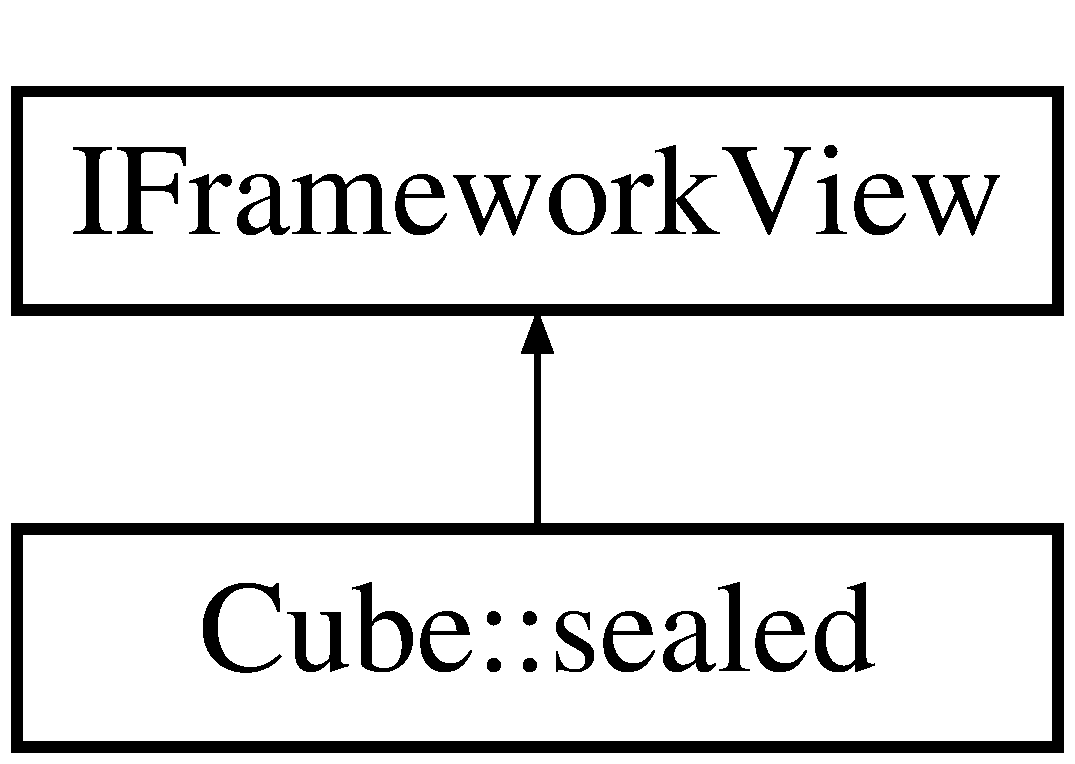
\includegraphics[height=2.000000cm]{class_cube_1_1sealed}
\end{center}
\end{figure}
\subsection*{Public Member Functions}
\begin{DoxyCompactItemize}
\item 
\hyperlink{class_cube_1_1sealed_a2921e740241bae7484e2682f90749b4f}{App} ()
\item 
virtual void \hyperlink{class_cube_1_1sealed_a9558710bf2600718f1ff7cbbcaa6213e}{Initialize} (Windows\+::\+Application\+Model\+::\+Core\+::\+Core\+Application\+View$^\wedge$ application\+View)
\item 
virtual void \hyperlink{class_cube_1_1sealed_aa548d90b484cc7e465459cf6a0635c6e}{Set\+Window} (Windows\+::\+U\+I\+::\+Core\+::\+Core\+Window$^\wedge$ window)
\item 
virtual void \hyperlink{class_cube_1_1sealed_a6b0578eb7635f4beda03ff766bf2b043}{Load} (Platform\+::\+String$^\wedge$ entry\+Point)
\item 
virtual void \hyperlink{class_cube_1_1sealed_a08467aa423e2a57ac7d9fd46f1b8e4ed}{Run} ()
\item 
virtual void \hyperlink{class_cube_1_1sealed_ad8675c3ad9633b9220384db60c6c2d15}{Uninitialize} ()
\end{DoxyCompactItemize}
\subsection*{Protected Member Functions}
\begin{DoxyCompactItemize}
\item 
void \hyperlink{class_cube_1_1sealed_a7bfa5f48c7415394b76a4152b5fb6abf}{On\+Activated} (Windows\+::\+Application\+Model\+::\+Core\+::\+Core\+Application\+View$^\wedge$ application\+View, Windows\+::\+Application\+Model\+::\+Activation\+::\+I\+Activated\+Event\+Args$^\wedge$ args)
\item 
void \hyperlink{class_cube_1_1sealed_a45dbe3797567e448ec7b26db0f30ea56}{On\+Suspending} (Platform\+::\+Object$^\wedge$ sender, Windows\+::\+Application\+Model\+::\+Suspending\+Event\+Args$^\wedge$ args)
\item 
void \hyperlink{class_cube_1_1sealed_a131584644dbd091d751a242b7a234922}{On\+Resuming} (Platform\+::\+Object$^\wedge$ sender, Platform\+::\+Object$^\wedge$ args)
\item 
void \hyperlink{class_cube_1_1sealed_accf4a33eb3419f7f81e564bf888846fc}{On\+Window\+Size\+Changed} (Windows\+::\+U\+I\+::\+Core\+::\+Core\+Window$^\wedge$ sender, Windows\+::\+U\+I\+::\+Core\+::\+Window\+Size\+Changed\+Event\+Args$^\wedge$ args)
\item 
void \hyperlink{class_cube_1_1sealed_aec9fe501363859f4c53a08f85c07db67}{On\+Visibility\+Changed} (Windows\+::\+U\+I\+::\+Core\+::\+Core\+Window$^\wedge$ sender, Windows\+::\+U\+I\+::\+Core\+::\+Visibility\+Changed\+Event\+Args$^\wedge$ args)
\item 
void \hyperlink{class_cube_1_1sealed_ac8edc3442699dcdcd40b235a8d8ab906}{On\+Window\+Closed} (Windows\+::\+U\+I\+::\+Core\+::\+Core\+Window$^\wedge$ sender, Windows\+::\+U\+I\+::\+Core\+::\+Core\+Window\+Event\+Args$^\wedge$ args)
\item 
void \hyperlink{class_cube_1_1sealed_a4621df1969e0c25abcaf42b9b09c1294}{On\+Dpi\+Changed} (Windows\+::\+Graphics\+::\+Display\+::\+Display\+Information$^\wedge$ sender, Platform\+::\+Object$^\wedge$ args)
\item 
void \hyperlink{class_cube_1_1sealed_a6c53f2260bcb4d51d1e4c21df620dbe0}{On\+Orientation\+Changed} (Windows\+::\+Graphics\+::\+Display\+::\+Display\+Information$^\wedge$ sender, Platform\+::\+Object$^\wedge$ args)
\item 
void \hyperlink{class_cube_1_1sealed_a46527bc6fafc0e7ca68c97d3cc2a51d4}{On\+Display\+Contents\+Invalidated} (Windows\+::\+Graphics\+::\+Display\+::\+Display\+Information$^\wedge$ sender, Platform\+::\+Object$^\wedge$ args)
\end{DoxyCompactItemize}


\subsection{Member Function Documentation}
\mbox{\Hypertarget{class_cube_1_1sealed_a2921e740241bae7484e2682f90749b4f}\label{class_cube_1_1sealed_a2921e740241bae7484e2682f90749b4f}} 
\index{Cube\+::sealed@{Cube\+::sealed}!App@{App}}
\index{App@{App}!Cube\+::sealed@{Cube\+::sealed}}
\subsubsection{\texorpdfstring{App()}{App()}}
{\footnotesize\ttfamily Cube\+::sealed\+::\+App (\begin{DoxyParamCaption}{ }\end{DoxyParamCaption})}

\mbox{\Hypertarget{class_cube_1_1sealed_a9558710bf2600718f1ff7cbbcaa6213e}\label{class_cube_1_1sealed_a9558710bf2600718f1ff7cbbcaa6213e}} 
\index{Cube\+::sealed@{Cube\+::sealed}!Initialize@{Initialize}}
\index{Initialize@{Initialize}!Cube\+::sealed@{Cube\+::sealed}}
\subsubsection{\texorpdfstring{Initialize()}{Initialize()}}
{\footnotesize\ttfamily virtual void Cube\+::sealed\+::\+Initialize (\begin{DoxyParamCaption}\item[{Windows\+::\+Application\+Model\+::\+Core\+::\+Core\+Application\+View$^\wedge$}]{application\+View }\end{DoxyParamCaption})\hspace{0.3cm}{\ttfamily [virtual]}}

\mbox{\Hypertarget{class_cube_1_1sealed_a6b0578eb7635f4beda03ff766bf2b043}\label{class_cube_1_1sealed_a6b0578eb7635f4beda03ff766bf2b043}} 
\index{Cube\+::sealed@{Cube\+::sealed}!Load@{Load}}
\index{Load@{Load}!Cube\+::sealed@{Cube\+::sealed}}
\subsubsection{\texorpdfstring{Load()}{Load()}}
{\footnotesize\ttfamily virtual void Cube\+::sealed\+::\+Load (\begin{DoxyParamCaption}\item[{Platform\+::\+String$^\wedge$}]{entry\+Point }\end{DoxyParamCaption})\hspace{0.3cm}{\ttfamily [virtual]}}

\mbox{\Hypertarget{class_cube_1_1sealed_a7bfa5f48c7415394b76a4152b5fb6abf}\label{class_cube_1_1sealed_a7bfa5f48c7415394b76a4152b5fb6abf}} 
\index{Cube\+::sealed@{Cube\+::sealed}!On\+Activated@{On\+Activated}}
\index{On\+Activated@{On\+Activated}!Cube\+::sealed@{Cube\+::sealed}}
\subsubsection{\texorpdfstring{On\+Activated()}{OnActivated()}}
{\footnotesize\ttfamily void Cube\+::sealed\+::\+On\+Activated (\begin{DoxyParamCaption}\item[{Windows\+::\+Application\+Model\+::\+Core\+::\+Core\+Application\+View$^\wedge$}]{application\+View,  }\item[{Windows\+::\+Application\+Model\+::\+Activation\+::\+I\+Activated\+Event\+Args$^\wedge$}]{args }\end{DoxyParamCaption})\hspace{0.3cm}{\ttfamily [protected]}}

\mbox{\Hypertarget{class_cube_1_1sealed_a46527bc6fafc0e7ca68c97d3cc2a51d4}\label{class_cube_1_1sealed_a46527bc6fafc0e7ca68c97d3cc2a51d4}} 
\index{Cube\+::sealed@{Cube\+::sealed}!On\+Display\+Contents\+Invalidated@{On\+Display\+Contents\+Invalidated}}
\index{On\+Display\+Contents\+Invalidated@{On\+Display\+Contents\+Invalidated}!Cube\+::sealed@{Cube\+::sealed}}
\subsubsection{\texorpdfstring{On\+Display\+Contents\+Invalidated()}{OnDisplayContentsInvalidated()}}
{\footnotesize\ttfamily void Cube\+::sealed\+::\+On\+Display\+Contents\+Invalidated (\begin{DoxyParamCaption}\item[{Windows\+::\+Graphics\+::\+Display\+::\+Display\+Information$^\wedge$}]{sender,  }\item[{Platform\+::\+Object$^\wedge$}]{args }\end{DoxyParamCaption})\hspace{0.3cm}{\ttfamily [protected]}}

\mbox{\Hypertarget{class_cube_1_1sealed_a4621df1969e0c25abcaf42b9b09c1294}\label{class_cube_1_1sealed_a4621df1969e0c25abcaf42b9b09c1294}} 
\index{Cube\+::sealed@{Cube\+::sealed}!On\+Dpi\+Changed@{On\+Dpi\+Changed}}
\index{On\+Dpi\+Changed@{On\+Dpi\+Changed}!Cube\+::sealed@{Cube\+::sealed}}
\subsubsection{\texorpdfstring{On\+Dpi\+Changed()}{OnDpiChanged()}}
{\footnotesize\ttfamily void Cube\+::sealed\+::\+On\+Dpi\+Changed (\begin{DoxyParamCaption}\item[{Windows\+::\+Graphics\+::\+Display\+::\+Display\+Information$^\wedge$}]{sender,  }\item[{Platform\+::\+Object$^\wedge$}]{args }\end{DoxyParamCaption})\hspace{0.3cm}{\ttfamily [protected]}}

\mbox{\Hypertarget{class_cube_1_1sealed_a6c53f2260bcb4d51d1e4c21df620dbe0}\label{class_cube_1_1sealed_a6c53f2260bcb4d51d1e4c21df620dbe0}} 
\index{Cube\+::sealed@{Cube\+::sealed}!On\+Orientation\+Changed@{On\+Orientation\+Changed}}
\index{On\+Orientation\+Changed@{On\+Orientation\+Changed}!Cube\+::sealed@{Cube\+::sealed}}
\subsubsection{\texorpdfstring{On\+Orientation\+Changed()}{OnOrientationChanged()}}
{\footnotesize\ttfamily void Cube\+::sealed\+::\+On\+Orientation\+Changed (\begin{DoxyParamCaption}\item[{Windows\+::\+Graphics\+::\+Display\+::\+Display\+Information$^\wedge$}]{sender,  }\item[{Platform\+::\+Object$^\wedge$}]{args }\end{DoxyParamCaption})\hspace{0.3cm}{\ttfamily [protected]}}

\mbox{\Hypertarget{class_cube_1_1sealed_a131584644dbd091d751a242b7a234922}\label{class_cube_1_1sealed_a131584644dbd091d751a242b7a234922}} 
\index{Cube\+::sealed@{Cube\+::sealed}!On\+Resuming@{On\+Resuming}}
\index{On\+Resuming@{On\+Resuming}!Cube\+::sealed@{Cube\+::sealed}}
\subsubsection{\texorpdfstring{On\+Resuming()}{OnResuming()}}
{\footnotesize\ttfamily void Cube\+::sealed\+::\+On\+Resuming (\begin{DoxyParamCaption}\item[{Platform\+::\+Object$^\wedge$}]{sender,  }\item[{Platform\+::\+Object$^\wedge$}]{args }\end{DoxyParamCaption})\hspace{0.3cm}{\ttfamily [protected]}}

\mbox{\Hypertarget{class_cube_1_1sealed_a45dbe3797567e448ec7b26db0f30ea56}\label{class_cube_1_1sealed_a45dbe3797567e448ec7b26db0f30ea56}} 
\index{Cube\+::sealed@{Cube\+::sealed}!On\+Suspending@{On\+Suspending}}
\index{On\+Suspending@{On\+Suspending}!Cube\+::sealed@{Cube\+::sealed}}
\subsubsection{\texorpdfstring{On\+Suspending()}{OnSuspending()}}
{\footnotesize\ttfamily void Cube\+::sealed\+::\+On\+Suspending (\begin{DoxyParamCaption}\item[{Platform\+::\+Object$^\wedge$}]{sender,  }\item[{Windows\+::\+Application\+Model\+::\+Suspending\+Event\+Args$^\wedge$}]{args }\end{DoxyParamCaption})\hspace{0.3cm}{\ttfamily [protected]}}

\mbox{\Hypertarget{class_cube_1_1sealed_aec9fe501363859f4c53a08f85c07db67}\label{class_cube_1_1sealed_aec9fe501363859f4c53a08f85c07db67}} 
\index{Cube\+::sealed@{Cube\+::sealed}!On\+Visibility\+Changed@{On\+Visibility\+Changed}}
\index{On\+Visibility\+Changed@{On\+Visibility\+Changed}!Cube\+::sealed@{Cube\+::sealed}}
\subsubsection{\texorpdfstring{On\+Visibility\+Changed()}{OnVisibilityChanged()}}
{\footnotesize\ttfamily void Cube\+::sealed\+::\+On\+Visibility\+Changed (\begin{DoxyParamCaption}\item[{Windows\+::\+U\+I\+::\+Core\+::\+Core\+Window$^\wedge$}]{sender,  }\item[{Windows\+::\+U\+I\+::\+Core\+::\+Visibility\+Changed\+Event\+Args$^\wedge$}]{args }\end{DoxyParamCaption})\hspace{0.3cm}{\ttfamily [protected]}}

\mbox{\Hypertarget{class_cube_1_1sealed_ac8edc3442699dcdcd40b235a8d8ab906}\label{class_cube_1_1sealed_ac8edc3442699dcdcd40b235a8d8ab906}} 
\index{Cube\+::sealed@{Cube\+::sealed}!On\+Window\+Closed@{On\+Window\+Closed}}
\index{On\+Window\+Closed@{On\+Window\+Closed}!Cube\+::sealed@{Cube\+::sealed}}
\subsubsection{\texorpdfstring{On\+Window\+Closed()}{OnWindowClosed()}}
{\footnotesize\ttfamily void Cube\+::sealed\+::\+On\+Window\+Closed (\begin{DoxyParamCaption}\item[{Windows\+::\+U\+I\+::\+Core\+::\+Core\+Window$^\wedge$}]{sender,  }\item[{Windows\+::\+U\+I\+::\+Core\+::\+Core\+Window\+Event\+Args$^\wedge$}]{args }\end{DoxyParamCaption})\hspace{0.3cm}{\ttfamily [protected]}}

\mbox{\Hypertarget{class_cube_1_1sealed_accf4a33eb3419f7f81e564bf888846fc}\label{class_cube_1_1sealed_accf4a33eb3419f7f81e564bf888846fc}} 
\index{Cube\+::sealed@{Cube\+::sealed}!On\+Window\+Size\+Changed@{On\+Window\+Size\+Changed}}
\index{On\+Window\+Size\+Changed@{On\+Window\+Size\+Changed}!Cube\+::sealed@{Cube\+::sealed}}
\subsubsection{\texorpdfstring{On\+Window\+Size\+Changed()}{OnWindowSizeChanged()}}
{\footnotesize\ttfamily void Cube\+::sealed\+::\+On\+Window\+Size\+Changed (\begin{DoxyParamCaption}\item[{Windows\+::\+U\+I\+::\+Core\+::\+Core\+Window$^\wedge$}]{sender,  }\item[{Windows\+::\+U\+I\+::\+Core\+::\+Window\+Size\+Changed\+Event\+Args$^\wedge$}]{args }\end{DoxyParamCaption})\hspace{0.3cm}{\ttfamily [protected]}}

\mbox{\Hypertarget{class_cube_1_1sealed_a08467aa423e2a57ac7d9fd46f1b8e4ed}\label{class_cube_1_1sealed_a08467aa423e2a57ac7d9fd46f1b8e4ed}} 
\index{Cube\+::sealed@{Cube\+::sealed}!Run@{Run}}
\index{Run@{Run}!Cube\+::sealed@{Cube\+::sealed}}
\subsubsection{\texorpdfstring{Run()}{Run()}}
{\footnotesize\ttfamily virtual void Cube\+::sealed\+::\+Run (\begin{DoxyParamCaption}{ }\end{DoxyParamCaption})\hspace{0.3cm}{\ttfamily [virtual]}}

\mbox{\Hypertarget{class_cube_1_1sealed_aa548d90b484cc7e465459cf6a0635c6e}\label{class_cube_1_1sealed_aa548d90b484cc7e465459cf6a0635c6e}} 
\index{Cube\+::sealed@{Cube\+::sealed}!Set\+Window@{Set\+Window}}
\index{Set\+Window@{Set\+Window}!Cube\+::sealed@{Cube\+::sealed}}
\subsubsection{\texorpdfstring{Set\+Window()}{SetWindow()}}
{\footnotesize\ttfamily virtual void Cube\+::sealed\+::\+Set\+Window (\begin{DoxyParamCaption}\item[{Windows\+::\+U\+I\+::\+Core\+::\+Core\+Window$^\wedge$}]{window }\end{DoxyParamCaption})\hspace{0.3cm}{\ttfamily [virtual]}}

\mbox{\Hypertarget{class_cube_1_1sealed_ad8675c3ad9633b9220384db60c6c2d15}\label{class_cube_1_1sealed_ad8675c3ad9633b9220384db60c6c2d15}} 
\index{Cube\+::sealed@{Cube\+::sealed}!Uninitialize@{Uninitialize}}
\index{Uninitialize@{Uninitialize}!Cube\+::sealed@{Cube\+::sealed}}
\subsubsection{\texorpdfstring{Uninitialize()}{Uninitialize()}}
{\footnotesize\ttfamily virtual void Cube\+::sealed\+::\+Uninitialize (\begin{DoxyParamCaption}{ }\end{DoxyParamCaption})\hspace{0.3cm}{\ttfamily [virtual]}}



The documentation for this class was generated from the following file\+:\begin{DoxyCompactItemize}
\item 
\hyperlink{_app_8h}{App.\+h}\end{DoxyCompactItemize}

\hypertarget{classsealed}{}\section{sealed Class Reference}
\label{classsealed}\index{sealed@{sealed}}


{\ttfamily \#include $<$App.\+h$>$}

Inheritance diagram for sealed\+:\begin{figure}[H]
\begin{center}
\leavevmode
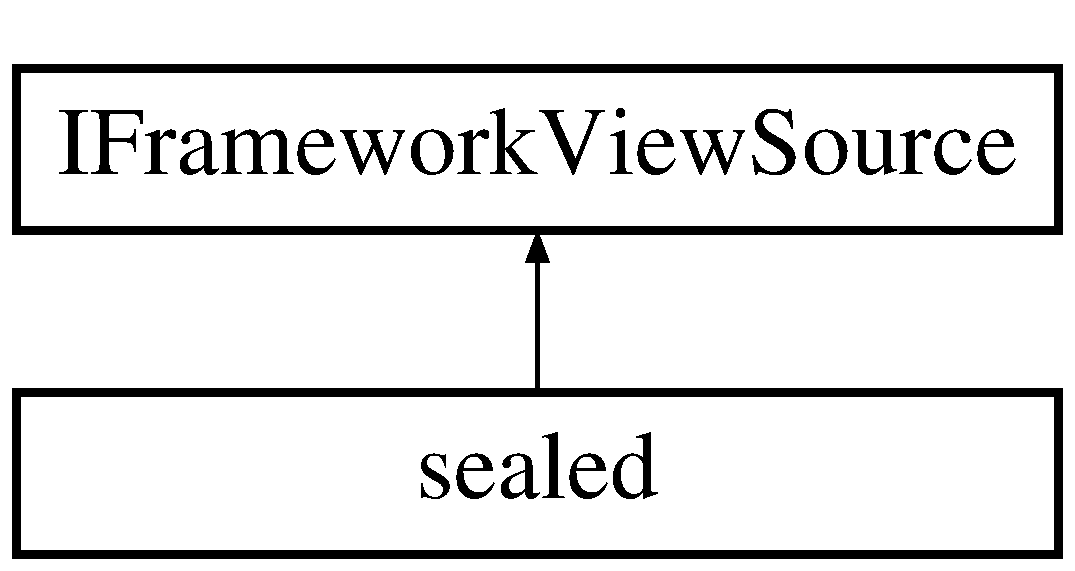
\includegraphics[height=2.000000cm]{classsealed}
\end{center}
\end{figure}
\subsection*{Public Member Functions}
\begin{DoxyCompactItemize}
\item 
virtual Windows\+::\+Application\+Model\+::\+Core\+::\+I\+Framework\+View \hyperlink{classsealed_ab46ae01be339d1457970df0de4f2ab76}{Create\+View} ()
\end{DoxyCompactItemize}


\subsection{Member Function Documentation}
\mbox{\Hypertarget{classsealed_ab46ae01be339d1457970df0de4f2ab76}\label{classsealed_ab46ae01be339d1457970df0de4f2ab76}} 
\index{sealed@{sealed}!Create\+View@{Create\+View}}
\index{Create\+View@{Create\+View}!sealed@{sealed}}
\subsubsection{\texorpdfstring{Create\+View()}{CreateView()}}
{\footnotesize\ttfamily virtual Windows\+::\+Application\+Model\+::\+Core\+::\+I\+Framework\+View sealed\+::\+Create\+View (\begin{DoxyParamCaption}{ }\end{DoxyParamCaption})\hspace{0.3cm}{\ttfamily [virtual]}}



The documentation for this class was generated from the following file\+:\begin{DoxyCompactItemize}
\item 
\hyperlink{_app_8h}{App.\+h}\end{DoxyCompactItemize}

\hypertarget{class_d_x_1_1_step_timer}{}\section{DX\+:\+:Step\+Timer Class Reference}
\label{class_d_x_1_1_step_timer}\index{D\+X\+::\+Step\+Timer@{D\+X\+::\+Step\+Timer}}


{\ttfamily \#include $<$Step\+Timer.\+h$>$}

\subsection*{Public Member Functions}
\begin{DoxyCompactItemize}
\item 
\hyperlink{class_d_x_1_1_step_timer_ae331f005f44c4e057c4bc7f96fe08f49}{Step\+Timer} ()
\item 
uint64 \hyperlink{class_d_x_1_1_step_timer_a311e3f7a1c0f1d8697f5aa68cadbc2f1}{Get\+Elapsed\+Ticks} () const
\item 
double \hyperlink{class_d_x_1_1_step_timer_a979be5067a77c50e31933ec12ca9b61b}{Get\+Elapsed\+Seconds} () const
\item 
uint64 \hyperlink{class_d_x_1_1_step_timer_a499065f09fb33708a1bc0c209d2f4792}{Get\+Total\+Ticks} () const
\item 
double \hyperlink{class_d_x_1_1_step_timer_a2c052574806156bdd31e88a31ef5f10f}{Get\+Total\+Seconds} () const
\item 
uint32 \hyperlink{class_d_x_1_1_step_timer_a0d20e64dea2ffd6cbe18fe84a62e7d44}{Get\+Frame\+Count} () const
\item 
uint32 \hyperlink{class_d_x_1_1_step_timer_a20dd186f3f67a26515bffca9081ff1dc}{Get\+Frames\+Per\+Second} () const
\item 
void \hyperlink{class_d_x_1_1_step_timer_ab108c5203686e605af494a4ebe39cb56}{Set\+Fixed\+Time\+Step} (bool is\+Fixed\+Timestep)
\item 
void \hyperlink{class_d_x_1_1_step_timer_ae026efbd3f030937bd5bd2d0326d825e}{Set\+Target\+Elapsed\+Ticks} (uint64 target\+Elapsed)
\item 
void \hyperlink{class_d_x_1_1_step_timer_a7487a7841823805904a548e3fa37cef2}{Set\+Target\+Elapsed\+Seconds} (double target\+Elapsed)
\item 
void \hyperlink{class_d_x_1_1_step_timer_ab07d4b15dec4b2ef390a359aeaad24fd}{Reset\+Elapsed\+Time} ()
\item 
{\footnotesize template$<$typename T\+Update $>$ }\\void \hyperlink{class_d_x_1_1_step_timer_a758b88f80e00fabee7167885476681ee}{Tick} (const T\+Update \&update)
\end{DoxyCompactItemize}
\subsection*{Static Public Member Functions}
\begin{DoxyCompactItemize}
\item 
static double \hyperlink{class_d_x_1_1_step_timer_a59a20b9b3294d930299991c62703b0d0}{Ticks\+To\+Seconds} (uint64 ticks)
\item 
static uint64 \hyperlink{class_d_x_1_1_step_timer_af6a26dd87202d9eeb167cc0b6e3c1a56}{Seconds\+To\+Ticks} (double seconds)
\end{DoxyCompactItemize}
\subsection*{Static Public Attributes}
\begin{DoxyCompactItemize}
\item 
static const uint64 \hyperlink{class_d_x_1_1_step_timer_aa671440c6c8008bd407ae889f5fb9f87}{Ticks\+Per\+Second} = 10000000
\end{DoxyCompactItemize}


\subsection{Constructor \& Destructor Documentation}
\mbox{\Hypertarget{class_d_x_1_1_step_timer_ae331f005f44c4e057c4bc7f96fe08f49}\label{class_d_x_1_1_step_timer_ae331f005f44c4e057c4bc7f96fe08f49}} 
\index{D\+X\+::\+Step\+Timer@{D\+X\+::\+Step\+Timer}!Step\+Timer@{Step\+Timer}}
\index{Step\+Timer@{Step\+Timer}!D\+X\+::\+Step\+Timer@{D\+X\+::\+Step\+Timer}}
\subsubsection{\texorpdfstring{Step\+Timer()}{StepTimer()}}
{\footnotesize\ttfamily D\+X\+::\+Step\+Timer\+::\+Step\+Timer (\begin{DoxyParamCaption}{ }\end{DoxyParamCaption})\hspace{0.3cm}{\ttfamily [inline]}}



\subsection{Member Function Documentation}
\mbox{\Hypertarget{class_d_x_1_1_step_timer_a979be5067a77c50e31933ec12ca9b61b}\label{class_d_x_1_1_step_timer_a979be5067a77c50e31933ec12ca9b61b}} 
\index{D\+X\+::\+Step\+Timer@{D\+X\+::\+Step\+Timer}!Get\+Elapsed\+Seconds@{Get\+Elapsed\+Seconds}}
\index{Get\+Elapsed\+Seconds@{Get\+Elapsed\+Seconds}!D\+X\+::\+Step\+Timer@{D\+X\+::\+Step\+Timer}}
\subsubsection{\texorpdfstring{Get\+Elapsed\+Seconds()}{GetElapsedSeconds()}}
{\footnotesize\ttfamily double D\+X\+::\+Step\+Timer\+::\+Get\+Elapsed\+Seconds (\begin{DoxyParamCaption}{ }\end{DoxyParamCaption}) const\hspace{0.3cm}{\ttfamily [inline]}}

\mbox{\Hypertarget{class_d_x_1_1_step_timer_a311e3f7a1c0f1d8697f5aa68cadbc2f1}\label{class_d_x_1_1_step_timer_a311e3f7a1c0f1d8697f5aa68cadbc2f1}} 
\index{D\+X\+::\+Step\+Timer@{D\+X\+::\+Step\+Timer}!Get\+Elapsed\+Ticks@{Get\+Elapsed\+Ticks}}
\index{Get\+Elapsed\+Ticks@{Get\+Elapsed\+Ticks}!D\+X\+::\+Step\+Timer@{D\+X\+::\+Step\+Timer}}
\subsubsection{\texorpdfstring{Get\+Elapsed\+Ticks()}{GetElapsedTicks()}}
{\footnotesize\ttfamily uint64 D\+X\+::\+Step\+Timer\+::\+Get\+Elapsed\+Ticks (\begin{DoxyParamCaption}{ }\end{DoxyParamCaption}) const\hspace{0.3cm}{\ttfamily [inline]}}

\mbox{\Hypertarget{class_d_x_1_1_step_timer_a0d20e64dea2ffd6cbe18fe84a62e7d44}\label{class_d_x_1_1_step_timer_a0d20e64dea2ffd6cbe18fe84a62e7d44}} 
\index{D\+X\+::\+Step\+Timer@{D\+X\+::\+Step\+Timer}!Get\+Frame\+Count@{Get\+Frame\+Count}}
\index{Get\+Frame\+Count@{Get\+Frame\+Count}!D\+X\+::\+Step\+Timer@{D\+X\+::\+Step\+Timer}}
\subsubsection{\texorpdfstring{Get\+Frame\+Count()}{GetFrameCount()}}
{\footnotesize\ttfamily uint32 D\+X\+::\+Step\+Timer\+::\+Get\+Frame\+Count (\begin{DoxyParamCaption}{ }\end{DoxyParamCaption}) const\hspace{0.3cm}{\ttfamily [inline]}}

\mbox{\Hypertarget{class_d_x_1_1_step_timer_a20dd186f3f67a26515bffca9081ff1dc}\label{class_d_x_1_1_step_timer_a20dd186f3f67a26515bffca9081ff1dc}} 
\index{D\+X\+::\+Step\+Timer@{D\+X\+::\+Step\+Timer}!Get\+Frames\+Per\+Second@{Get\+Frames\+Per\+Second}}
\index{Get\+Frames\+Per\+Second@{Get\+Frames\+Per\+Second}!D\+X\+::\+Step\+Timer@{D\+X\+::\+Step\+Timer}}
\subsubsection{\texorpdfstring{Get\+Frames\+Per\+Second()}{GetFramesPerSecond()}}
{\footnotesize\ttfamily uint32 D\+X\+::\+Step\+Timer\+::\+Get\+Frames\+Per\+Second (\begin{DoxyParamCaption}{ }\end{DoxyParamCaption}) const\hspace{0.3cm}{\ttfamily [inline]}}

\mbox{\Hypertarget{class_d_x_1_1_step_timer_a2c052574806156bdd31e88a31ef5f10f}\label{class_d_x_1_1_step_timer_a2c052574806156bdd31e88a31ef5f10f}} 
\index{D\+X\+::\+Step\+Timer@{D\+X\+::\+Step\+Timer}!Get\+Total\+Seconds@{Get\+Total\+Seconds}}
\index{Get\+Total\+Seconds@{Get\+Total\+Seconds}!D\+X\+::\+Step\+Timer@{D\+X\+::\+Step\+Timer}}
\subsubsection{\texorpdfstring{Get\+Total\+Seconds()}{GetTotalSeconds()}}
{\footnotesize\ttfamily double D\+X\+::\+Step\+Timer\+::\+Get\+Total\+Seconds (\begin{DoxyParamCaption}{ }\end{DoxyParamCaption}) const\hspace{0.3cm}{\ttfamily [inline]}}

\mbox{\Hypertarget{class_d_x_1_1_step_timer_a499065f09fb33708a1bc0c209d2f4792}\label{class_d_x_1_1_step_timer_a499065f09fb33708a1bc0c209d2f4792}} 
\index{D\+X\+::\+Step\+Timer@{D\+X\+::\+Step\+Timer}!Get\+Total\+Ticks@{Get\+Total\+Ticks}}
\index{Get\+Total\+Ticks@{Get\+Total\+Ticks}!D\+X\+::\+Step\+Timer@{D\+X\+::\+Step\+Timer}}
\subsubsection{\texorpdfstring{Get\+Total\+Ticks()}{GetTotalTicks()}}
{\footnotesize\ttfamily uint64 D\+X\+::\+Step\+Timer\+::\+Get\+Total\+Ticks (\begin{DoxyParamCaption}{ }\end{DoxyParamCaption}) const\hspace{0.3cm}{\ttfamily [inline]}}

\mbox{\Hypertarget{class_d_x_1_1_step_timer_ab07d4b15dec4b2ef390a359aeaad24fd}\label{class_d_x_1_1_step_timer_ab07d4b15dec4b2ef390a359aeaad24fd}} 
\index{D\+X\+::\+Step\+Timer@{D\+X\+::\+Step\+Timer}!Reset\+Elapsed\+Time@{Reset\+Elapsed\+Time}}
\index{Reset\+Elapsed\+Time@{Reset\+Elapsed\+Time}!D\+X\+::\+Step\+Timer@{D\+X\+::\+Step\+Timer}}
\subsubsection{\texorpdfstring{Reset\+Elapsed\+Time()}{ResetElapsedTime()}}
{\footnotesize\ttfamily void D\+X\+::\+Step\+Timer\+::\+Reset\+Elapsed\+Time (\begin{DoxyParamCaption}{ }\end{DoxyParamCaption})\hspace{0.3cm}{\ttfamily [inline]}}

\mbox{\Hypertarget{class_d_x_1_1_step_timer_af6a26dd87202d9eeb167cc0b6e3c1a56}\label{class_d_x_1_1_step_timer_af6a26dd87202d9eeb167cc0b6e3c1a56}} 
\index{D\+X\+::\+Step\+Timer@{D\+X\+::\+Step\+Timer}!Seconds\+To\+Ticks@{Seconds\+To\+Ticks}}
\index{Seconds\+To\+Ticks@{Seconds\+To\+Ticks}!D\+X\+::\+Step\+Timer@{D\+X\+::\+Step\+Timer}}
\subsubsection{\texorpdfstring{Seconds\+To\+Ticks()}{SecondsToTicks()}}
{\footnotesize\ttfamily static uint64 D\+X\+::\+Step\+Timer\+::\+Seconds\+To\+Ticks (\begin{DoxyParamCaption}\item[{double}]{seconds }\end{DoxyParamCaption})\hspace{0.3cm}{\ttfamily [inline]}, {\ttfamily [static]}}

\mbox{\Hypertarget{class_d_x_1_1_step_timer_ab108c5203686e605af494a4ebe39cb56}\label{class_d_x_1_1_step_timer_ab108c5203686e605af494a4ebe39cb56}} 
\index{D\+X\+::\+Step\+Timer@{D\+X\+::\+Step\+Timer}!Set\+Fixed\+Time\+Step@{Set\+Fixed\+Time\+Step}}
\index{Set\+Fixed\+Time\+Step@{Set\+Fixed\+Time\+Step}!D\+X\+::\+Step\+Timer@{D\+X\+::\+Step\+Timer}}
\subsubsection{\texorpdfstring{Set\+Fixed\+Time\+Step()}{SetFixedTimeStep()}}
{\footnotesize\ttfamily void D\+X\+::\+Step\+Timer\+::\+Set\+Fixed\+Time\+Step (\begin{DoxyParamCaption}\item[{bool}]{is\+Fixed\+Timestep }\end{DoxyParamCaption})\hspace{0.3cm}{\ttfamily [inline]}}

\mbox{\Hypertarget{class_d_x_1_1_step_timer_a7487a7841823805904a548e3fa37cef2}\label{class_d_x_1_1_step_timer_a7487a7841823805904a548e3fa37cef2}} 
\index{D\+X\+::\+Step\+Timer@{D\+X\+::\+Step\+Timer}!Set\+Target\+Elapsed\+Seconds@{Set\+Target\+Elapsed\+Seconds}}
\index{Set\+Target\+Elapsed\+Seconds@{Set\+Target\+Elapsed\+Seconds}!D\+X\+::\+Step\+Timer@{D\+X\+::\+Step\+Timer}}
\subsubsection{\texorpdfstring{Set\+Target\+Elapsed\+Seconds()}{SetTargetElapsedSeconds()}}
{\footnotesize\ttfamily void D\+X\+::\+Step\+Timer\+::\+Set\+Target\+Elapsed\+Seconds (\begin{DoxyParamCaption}\item[{double}]{target\+Elapsed }\end{DoxyParamCaption})\hspace{0.3cm}{\ttfamily [inline]}}

\mbox{\Hypertarget{class_d_x_1_1_step_timer_ae026efbd3f030937bd5bd2d0326d825e}\label{class_d_x_1_1_step_timer_ae026efbd3f030937bd5bd2d0326d825e}} 
\index{D\+X\+::\+Step\+Timer@{D\+X\+::\+Step\+Timer}!Set\+Target\+Elapsed\+Ticks@{Set\+Target\+Elapsed\+Ticks}}
\index{Set\+Target\+Elapsed\+Ticks@{Set\+Target\+Elapsed\+Ticks}!D\+X\+::\+Step\+Timer@{D\+X\+::\+Step\+Timer}}
\subsubsection{\texorpdfstring{Set\+Target\+Elapsed\+Ticks()}{SetTargetElapsedTicks()}}
{\footnotesize\ttfamily void D\+X\+::\+Step\+Timer\+::\+Set\+Target\+Elapsed\+Ticks (\begin{DoxyParamCaption}\item[{uint64}]{target\+Elapsed }\end{DoxyParamCaption})\hspace{0.3cm}{\ttfamily [inline]}}

\mbox{\Hypertarget{class_d_x_1_1_step_timer_a758b88f80e00fabee7167885476681ee}\label{class_d_x_1_1_step_timer_a758b88f80e00fabee7167885476681ee}} 
\index{D\+X\+::\+Step\+Timer@{D\+X\+::\+Step\+Timer}!Tick@{Tick}}
\index{Tick@{Tick}!D\+X\+::\+Step\+Timer@{D\+X\+::\+Step\+Timer}}
\subsubsection{\texorpdfstring{Tick()}{Tick()}}
{\footnotesize\ttfamily template$<$typename T\+Update $>$ \\
void D\+X\+::\+Step\+Timer\+::\+Tick (\begin{DoxyParamCaption}\item[{const T\+Update \&}]{update }\end{DoxyParamCaption})\hspace{0.3cm}{\ttfamily [inline]}}

\mbox{\Hypertarget{class_d_x_1_1_step_timer_a59a20b9b3294d930299991c62703b0d0}\label{class_d_x_1_1_step_timer_a59a20b9b3294d930299991c62703b0d0}} 
\index{D\+X\+::\+Step\+Timer@{D\+X\+::\+Step\+Timer}!Ticks\+To\+Seconds@{Ticks\+To\+Seconds}}
\index{Ticks\+To\+Seconds@{Ticks\+To\+Seconds}!D\+X\+::\+Step\+Timer@{D\+X\+::\+Step\+Timer}}
\subsubsection{\texorpdfstring{Ticks\+To\+Seconds()}{TicksToSeconds()}}
{\footnotesize\ttfamily static double D\+X\+::\+Step\+Timer\+::\+Ticks\+To\+Seconds (\begin{DoxyParamCaption}\item[{uint64}]{ticks }\end{DoxyParamCaption})\hspace{0.3cm}{\ttfamily [inline]}, {\ttfamily [static]}}



\subsection{Member Data Documentation}
\mbox{\Hypertarget{class_d_x_1_1_step_timer_aa671440c6c8008bd407ae889f5fb9f87}\label{class_d_x_1_1_step_timer_aa671440c6c8008bd407ae889f5fb9f87}} 
\index{D\+X\+::\+Step\+Timer@{D\+X\+::\+Step\+Timer}!Ticks\+Per\+Second@{Ticks\+Per\+Second}}
\index{Ticks\+Per\+Second@{Ticks\+Per\+Second}!D\+X\+::\+Step\+Timer@{D\+X\+::\+Step\+Timer}}
\subsubsection{\texorpdfstring{Ticks\+Per\+Second}{TicksPerSecond}}
{\footnotesize\ttfamily const uint64 D\+X\+::\+Step\+Timer\+::\+Ticks\+Per\+Second = 10000000\hspace{0.3cm}{\ttfamily [static]}}



The documentation for this class was generated from the following file\+:\begin{DoxyCompactItemize}
\item 
Common/\hyperlink{_step_timer_8h}{Step\+Timer.\+h}\end{DoxyCompactItemize}

\hypertarget{struct_cube_1_1_vertex_position_color}{}\section{Cube\+:\+:Vertex\+Position\+Color Struct Reference}
\label{struct_cube_1_1_vertex_position_color}\index{Cube\+::\+Vertex\+Position\+Color@{Cube\+::\+Vertex\+Position\+Color}}


{\ttfamily \#include $<$Shader\+Structures.\+h$>$}

\subsection*{Public Attributes}
\begin{DoxyCompactItemize}
\item 
Direct\+X\+::\+X\+M\+F\+L\+O\+A\+T3 \hyperlink{struct_cube_1_1_vertex_position_color_a39315affdd120bca4aa0c38d0d354427}{pos}
\item 
Direct\+X\+::\+X\+M\+F\+L\+O\+A\+T3 \hyperlink{struct_cube_1_1_vertex_position_color_aaeb8e604e74dbf92a7becaa154557a0a}{normal}
\end{DoxyCompactItemize}


\subsection{Member Data Documentation}
\mbox{\Hypertarget{struct_cube_1_1_vertex_position_color_aaeb8e604e74dbf92a7becaa154557a0a}\label{struct_cube_1_1_vertex_position_color_aaeb8e604e74dbf92a7becaa154557a0a}} 
\index{Cube\+::\+Vertex\+Position\+Color@{Cube\+::\+Vertex\+Position\+Color}!normal@{normal}}
\index{normal@{normal}!Cube\+::\+Vertex\+Position\+Color@{Cube\+::\+Vertex\+Position\+Color}}
\subsubsection{\texorpdfstring{normal}{normal}}
{\footnotesize\ttfamily Direct\+X\+::\+X\+M\+F\+L\+O\+A\+T3 Cube\+::\+Vertex\+Position\+Color\+::normal}

\mbox{\Hypertarget{struct_cube_1_1_vertex_position_color_a39315affdd120bca4aa0c38d0d354427}\label{struct_cube_1_1_vertex_position_color_a39315affdd120bca4aa0c38d0d354427}} 
\index{Cube\+::\+Vertex\+Position\+Color@{Cube\+::\+Vertex\+Position\+Color}!pos@{pos}}
\index{pos@{pos}!Cube\+::\+Vertex\+Position\+Color@{Cube\+::\+Vertex\+Position\+Color}}
\subsubsection{\texorpdfstring{pos}{pos}}
{\footnotesize\ttfamily Direct\+X\+::\+X\+M\+F\+L\+O\+A\+T3 Cube\+::\+Vertex\+Position\+Color\+::pos}



The documentation for this struct was generated from the following file\+:\begin{DoxyCompactItemize}
\item 
Content/\hyperlink{_shader_structures_8h}{Shader\+Structures.\+h}\end{DoxyCompactItemize}

\chapter{File Documentation}
\hypertarget{_app_8cpp}{}\section{App.\+cpp File Reference}
\label{_app_8cpp}\index{App.\+cpp@{App.\+cpp}}
{\ttfamily \#include \char`\"{}pch.\+h\char`\"{}}\newline
{\ttfamily \#include \char`\"{}App.\+h\char`\"{}}\newline
{\ttfamily \#include $<$ppltasks.\+h$>$}\newline
\subsection*{Functions}
\begin{DoxyCompactItemize}
\item 
int \hyperlink{_app_8cpp_a7099d6364756ad49d8413160485ada39}{main} (Platform\+::\+Array$<$ Platform\+::\+String$^\wedge$$>$$^\wedge$)
\end{DoxyCompactItemize}


\subsection{Function Documentation}
\mbox{\Hypertarget{_app_8cpp_a7099d6364756ad49d8413160485ada39}\label{_app_8cpp_a7099d6364756ad49d8413160485ada39}} 
\index{App.\+cpp@{App.\+cpp}!main@{main}}
\index{main@{main}!App.\+cpp@{App.\+cpp}}
\subsubsection{\texorpdfstring{main()}{main()}}
{\footnotesize\ttfamily int main (\begin{DoxyParamCaption}\item[{Platform\+::\+Array$<$ Platform\+::\+String$^\wedge$$>$$^\wedge$}]{ }\end{DoxyParamCaption})}


\hypertarget{_app_8h}{}\section{App.\+h File Reference}
\label{_app_8h}\index{App.\+h@{App.\+h}}
{\ttfamily \#include \char`\"{}pch.\+h\char`\"{}}\newline
{\ttfamily \#include \char`\"{}Common\textbackslash{}\+Device\+Resources.\+h\char`\"{}}\newline
{\ttfamily \#include \char`\"{}Cube\+Main.\+h\char`\"{}}\newline
\subsection*{Classes}
\begin{DoxyCompactItemize}
\item 
class \hyperlink{class_cube_1_1sealed}{Cube\+::sealed}
\item 
class \hyperlink{classsealed}{sealed}
\end{DoxyCompactItemize}
\subsection*{Namespaces}
\begin{DoxyCompactItemize}
\item 
 \hyperlink{namespace_cube}{Cube}
\end{DoxyCompactItemize}

\hypertarget{_device_resources_8cpp}{}\section{Common/\+Device\+Resources.cpp File Reference}
\label{_device_resources_8cpp}\index{Common/\+Device\+Resources.\+cpp@{Common/\+Device\+Resources.\+cpp}}
{\ttfamily \#include \char`\"{}pch.\+h\char`\"{}}\newline
{\ttfamily \#include \char`\"{}Device\+Resources.\+h\char`\"{}}\newline
{\ttfamily \#include \char`\"{}Direct\+X\+Helper.\+h\char`\"{}}\newline
\subsection*{Namespaces}
\begin{DoxyCompactItemize}
\item 
 \hyperlink{namespace_display_metrics}{Display\+Metrics}
\item 
 \hyperlink{namespace_screen_rotation}{Screen\+Rotation}
\end{DoxyCompactItemize}

\hypertarget{_device_resources_8h}{}\section{Common/\+Device\+Resources.h File Reference}
\label{_device_resources_8h}\index{Common/\+Device\+Resources.\+h@{Common/\+Device\+Resources.\+h}}
\subsection*{Classes}
\begin{DoxyCompactItemize}
\item 
class \hyperlink{class_d_x_1_1_device_resources}{D\+X\+::\+Device\+Resources}
\end{DoxyCompactItemize}
\subsection*{Namespaces}
\begin{DoxyCompactItemize}
\item 
 \hyperlink{namespace_d_x}{DX}
\end{DoxyCompactItemize}
\subsection*{Functions}
\begin{DoxyCompactItemize}
\item 
virtual void \hyperlink{namespace_d_x_af35cc4f32a0b9c196ec7810fe1ec458c}{D\+X\+::\+On\+Device\+Restored} ()=0
\end{DoxyCompactItemize}

\hypertarget{_direct_x_helper_8h}{}\section{Common/\+Direct\+X\+Helper.h File Reference}
\label{_direct_x_helper_8h}\index{Common/\+Direct\+X\+Helper.\+h@{Common/\+Direct\+X\+Helper.\+h}}
{\ttfamily \#include $<$ppltasks.\+h$>$}\newline
\subsection*{Namespaces}
\begin{DoxyCompactItemize}
\item 
 \hyperlink{namespace_d_x}{DX}
\end{DoxyCompactItemize}
\subsection*{Functions}
\begin{DoxyCompactItemize}
\item 
void \hyperlink{namespace_d_x_aa15dd958b09a7ddbfdf9f4c34d2e8f52}{D\+X\+::\+Throw\+If\+Failed} (H\+R\+E\+S\+U\+LT hr)
\item 
Concurrency\+::task$<$ std\+::vector$<$ byte $>$ $>$ \hyperlink{namespace_d_x_a51d84a785c28e9e6ababf8a5d0118037}{D\+X\+::\+Read\+Data\+Async} (const std\+::wstring \&filename)
\item 
float \hyperlink{namespace_d_x_ab445f4cbfd345e67c629c9f59b696a74}{D\+X\+::\+Convert\+Dips\+To\+Pixels} (float dips, float dpi)
\end{DoxyCompactItemize}

\hypertarget{_step_timer_8h}{}\section{Common/\+Step\+Timer.h File Reference}
\label{_step_timer_8h}\index{Common/\+Step\+Timer.\+h@{Common/\+Step\+Timer.\+h}}
{\ttfamily \#include $<$wrl.\+h$>$}\newline
\subsection*{Classes}
\begin{DoxyCompactItemize}
\item 
class \hyperlink{class_d_x_1_1_step_timer}{D\+X\+::\+Step\+Timer}
\end{DoxyCompactItemize}
\subsection*{Namespaces}
\begin{DoxyCompactItemize}
\item 
 \hyperlink{namespace_d_x}{DX}
\end{DoxyCompactItemize}

\hypertarget{_sample3_d_scene_renderer_8cpp}{}\section{Content/\+Sample3\+D\+Scene\+Renderer.cpp File Reference}
\label{_sample3_d_scene_renderer_8cpp}\index{Content/\+Sample3\+D\+Scene\+Renderer.\+cpp@{Content/\+Sample3\+D\+Scene\+Renderer.\+cpp}}
{\ttfamily \#include \char`\"{}pch.\+h\char`\"{}}\newline
{\ttfamily \#include \char`\"{}Sample3\+D\+Scene\+Renderer.\+h\char`\"{}}\newline
{\ttfamily \#include \char`\"{}D\+D\+S\+Texture\+Loader.\+h\char`\"{}}\newline
{\ttfamily \#include \char`\"{}Model.\+h\char`\"{}}\newline
{\ttfamily \#include \char`\"{}..\textbackslash{}\+Common\textbackslash{}\+Direct\+X\+Helper.\+h\char`\"{}}\newline

\hypertarget{_sample3_d_scene_renderer_8h}{}\section{Content/\+Sample3\+D\+Scene\+Renderer.h File Reference}
\label{_sample3_d_scene_renderer_8h}\index{Content/\+Sample3\+D\+Scene\+Renderer.\+h@{Content/\+Sample3\+D\+Scene\+Renderer.\+h}}
{\ttfamily \#include \char`\"{}..\textbackslash{}\+Common\textbackslash{}\+Device\+Resources.\+h\char`\"{}}\newline
{\ttfamily \#include \char`\"{}Shader\+Structures.\+h\char`\"{}}\newline
{\ttfamily \#include \char`\"{}..\textbackslash{}\+Common\textbackslash{}\+Step\+Timer.\+h\char`\"{}}\newline
\subsection*{Classes}
\begin{DoxyCompactItemize}
\item 
class \hyperlink{class_cube_1_1_sample3_d_scene_renderer}{Cube\+::\+Sample3\+D\+Scene\+Renderer}
\end{DoxyCompactItemize}
\subsection*{Namespaces}
\begin{DoxyCompactItemize}
\item 
 \hyperlink{namespace_cube}{Cube}
\end{DoxyCompactItemize}

\hypertarget{_sample_fps_text_renderer_8cpp}{}\section{Content/\+Sample\+Fps\+Text\+Renderer.cpp File Reference}
\label{_sample_fps_text_renderer_8cpp}\index{Content/\+Sample\+Fps\+Text\+Renderer.\+cpp@{Content/\+Sample\+Fps\+Text\+Renderer.\+cpp}}
{\ttfamily \#include \char`\"{}pch.\+h\char`\"{}}\newline
{\ttfamily \#include \char`\"{}Sample\+Fps\+Text\+Renderer.\+h\char`\"{}}\newline
{\ttfamily \#include \char`\"{}Common/\+Direct\+X\+Helper.\+h\char`\"{}}\newline

\hypertarget{_sample_fps_text_renderer_8h}{}\section{Content/\+Sample\+Fps\+Text\+Renderer.h File Reference}
\label{_sample_fps_text_renderer_8h}\index{Content/\+Sample\+Fps\+Text\+Renderer.\+h@{Content/\+Sample\+Fps\+Text\+Renderer.\+h}}
{\ttfamily \#include $<$string$>$}\newline
{\ttfamily \#include \char`\"{}..\textbackslash{}\+Common\textbackslash{}\+Device\+Resources.\+h\char`\"{}}\newline
{\ttfamily \#include \char`\"{}..\textbackslash{}\+Common\textbackslash{}\+Step\+Timer.\+h\char`\"{}}\newline
\subsection*{Classes}
\begin{DoxyCompactItemize}
\item 
class \hyperlink{class_cube_1_1_sample_fps_text_renderer}{Cube\+::\+Sample\+Fps\+Text\+Renderer}
\end{DoxyCompactItemize}
\subsection*{Namespaces}
\begin{DoxyCompactItemize}
\item 
 \hyperlink{namespace_cube}{Cube}
\end{DoxyCompactItemize}

\hypertarget{_shader_structures_8h}{}\section{Content/\+Shader\+Structures.h File Reference}
\label{_shader_structures_8h}\index{Content/\+Shader\+Structures.\+h@{Content/\+Shader\+Structures.\+h}}
\subsection*{Classes}
\begin{DoxyCompactItemize}
\item 
struct \hyperlink{struct_cube_1_1_model_view_projection_constant_buffer}{Cube\+::\+Model\+View\+Projection\+Constant\+Buffer}
\item 
struct \hyperlink{struct_cube_1_1_vertex_position_color}{Cube\+::\+Vertex\+Position\+Color}
\end{DoxyCompactItemize}
\subsection*{Namespaces}
\begin{DoxyCompactItemize}
\item 
 \hyperlink{namespace_cube}{Cube}
\end{DoxyCompactItemize}

\hypertarget{_cube_main_8cpp}{}\section{Cube\+Main.\+cpp File Reference}
\label{_cube_main_8cpp}\index{Cube\+Main.\+cpp@{Cube\+Main.\+cpp}}
{\ttfamily \#include \char`\"{}pch.\+h\char`\"{}}\newline
{\ttfamily \#include \char`\"{}Cube\+Main.\+h\char`\"{}}\newline
{\ttfamily \#include \char`\"{}Common\textbackslash{}\+Direct\+X\+Helper.\+h\char`\"{}}\newline

\hypertarget{_cube_main_8h}{}\section{Cube\+Main.\+h File Reference}
\label{_cube_main_8h}\index{Cube\+Main.\+h@{Cube\+Main.\+h}}
{\ttfamily \#include \char`\"{}Common\textbackslash{}\+Step\+Timer.\+h\char`\"{}}\newline
{\ttfamily \#include \char`\"{}Common\textbackslash{}\+Device\+Resources.\+h\char`\"{}}\newline
{\ttfamily \#include \char`\"{}Content\textbackslash{}\+Sample3\+D\+Scene\+Renderer.\+h\char`\"{}}\newline
{\ttfamily \#include \char`\"{}Content\textbackslash{}\+Sample\+Fps\+Text\+Renderer.\+h\char`\"{}}\newline
\subsection*{Classes}
\begin{DoxyCompactItemize}
\item 
class \hyperlink{class_cube_1_1_cube_main}{Cube\+::\+Cube\+Main}
\end{DoxyCompactItemize}
\subsection*{Namespaces}
\begin{DoxyCompactItemize}
\item 
 \hyperlink{namespace_cube}{Cube}
\end{DoxyCompactItemize}

\hypertarget{_mesh_obj_8cpp}{}\section{Mesh\+Obj.\+cpp File Reference}
\label{_mesh_obj_8cpp}\index{Mesh\+Obj.\+cpp@{Mesh\+Obj.\+cpp}}
{\ttfamily \#include \char`\"{}pch.\+h\char`\"{}}\newline

\hypertarget{_mesh_obj_8h}{}\section{Mesh\+Obj.\+h File Reference}
\label{_mesh_obj_8h}\index{Mesh\+Obj.\+h@{Mesh\+Obj.\+h}}

\hypertarget{pch_8cpp}{}\section{pch.\+cpp File Reference}
\label{pch_8cpp}\index{pch.\+cpp@{pch.\+cpp}}
{\ttfamily \#include \char`\"{}pch.\+h\char`\"{}}\newline

\hypertarget{pch_8h}{}\section{pch.\+h File Reference}
\label{pch_8h}\index{pch.\+h@{pch.\+h}}
{\ttfamily \#include $<$wrl.\+h$>$}\newline
{\ttfamily \#include $<$wrl/client.\+h$>$}\newline
{\ttfamily \#include $<$dxgi1\+\_\+4.\+h$>$}\newline
{\ttfamily \#include $<$d3d11\+\_\+3.\+h$>$}\newline
{\ttfamily \#include $<$d2d1\+\_\+3.\+h$>$}\newline
{\ttfamily \#include $<$d2d1effects\+\_\+2.\+h$>$}\newline
{\ttfamily \#include $<$dwrite\+\_\+3.\+h$>$}\newline
{\ttfamily \#include $<$wincodec.\+h$>$}\newline
{\ttfamily \#include $<$Direct\+X\+Colors.\+h$>$}\newline
{\ttfamily \#include $<$Direct\+X\+Math.\+h$>$}\newline
{\ttfamily \#include $<$memory$>$}\newline
{\ttfamily \#include $<$agile.\+h$>$}\newline
{\ttfamily \#include $<$concrt.\+h$>$}\newline

%--- End generated contents ---

% Index
\backmatter
\newpage
\phantomsection
\clearemptydoublepage
\addcontentsline{toc}{chapter}{Index}
\printindex

\end{document}
